\chapter{面向高动态水下场景的相干 AFDM-IM 传输方案}
\label{chap:coherent_afdm_im}

面向高动态水下通信需求，UWOC 链路正由低动态准静态应用逐步向高速机动、强时变场景扩展\cite{hoeherUnderwaterOpticalWireless2021, MianXiangUUVJiQunYingYongDeShuiXiaWuXianGuangTongXinGuanJianJiShu2025}。在此类条件下，平台相对运动引起的多普勒频移会破坏传统 OFDM 子载波正交关系，导致严重载波间干扰\cite{zhuDopplerResistantOrthogonalChirp2022, fernandesDigitallyMitigatingDoppler2023}；同时，相干接收架构中发射与本振激光器的有限线宽还将引入维纳相位噪声\cite{tangUnderwaterCoherentOptical2021, huPerformanceCoherentOptical2025}，使接收端面临多普勒扩展与相位漂移的联合失真。传统 IM-DD 多载波体制由于仅能利用光强维度，难以同时兼顾接收灵敏度、抗多普勒能力与高阶调制需求\cite{liuMultiDegreeofFreedomUnderwaterOptical2022}。

AFDM 基于 DAFT 构造正交啁啾基函数，使时延与多普勒扩展在等效表示域中呈现结构性耦合形式，在双选择性信道中具有显著的鲁棒性优势\cite{bemaniAFDMFullDiversity2021, taoAffineFrequencyDivision2025}。相干探测能够恢复信号的幅度与相位信息，在接收灵敏度与背景噪声抑制方面具有优势，更适合支撑复数域 AFDM 传输\cite{guiomarCoherentFreeSpaceOptical2022, huPerformanceCoherentOptical2025}。在此基础上引入索引调制机制，通过激活位置与星座符号联合承载信息，可在提高比特映射效率的同时引入块稀疏结构\cite{basarOrthogonalFrequencyDivision2013, taoAffineFrequencyDivision2025}。更重要的是，AFDM-IM 中天然存在的大量未激活位置在理想情况下应保持为零，这些静默位置不仅服务于索引信息传输，还能够在接收端转化为可用于残余频偏感知的隐式结构参考，使索引调制从单纯的频谱效率提升工具进一步演化为接收端结构自感知的波形设计资源。

基于上述分析，本文提出相干 AFDM-IM 传输方案，建立包含多径、多普勒频移与维纳相位噪声的系统模型，推导 DAFT 域等效输入输出关系；进一步利用 AFDM-IM 静默位置所蕴含的零结构先验，研究基于静默位置泄露能量最小化与稀疏度量驱动的盲/半盲残余 CFO 补偿与检测方法。该思路将 IM 从单纯增谱效工具提升为接收端结构自感知资源，在减少显式导频开销的同时提高系统对残余频偏失配的适应能力，并对维纳相位噪声实现鲁棒容忍。

\section{相干 AFDM-IM 系统模型构建}
\label{sec:coherent_afdm_im_model}

本节在第二章双选择性信道模型与 AFDM 基本原理基础上，建立相干 AFDM-IM 系统的发射端、信道与接收端模型。系统完整框图如图~\ref{fig:coherent_afdm_im_system} 所示。与第三章的 ACO-AFDM 方案不同，本章采用相干光架构直接传输复数域 AFDM-IM 基带信号。

\begin{figure}[htbp]
    \centering
    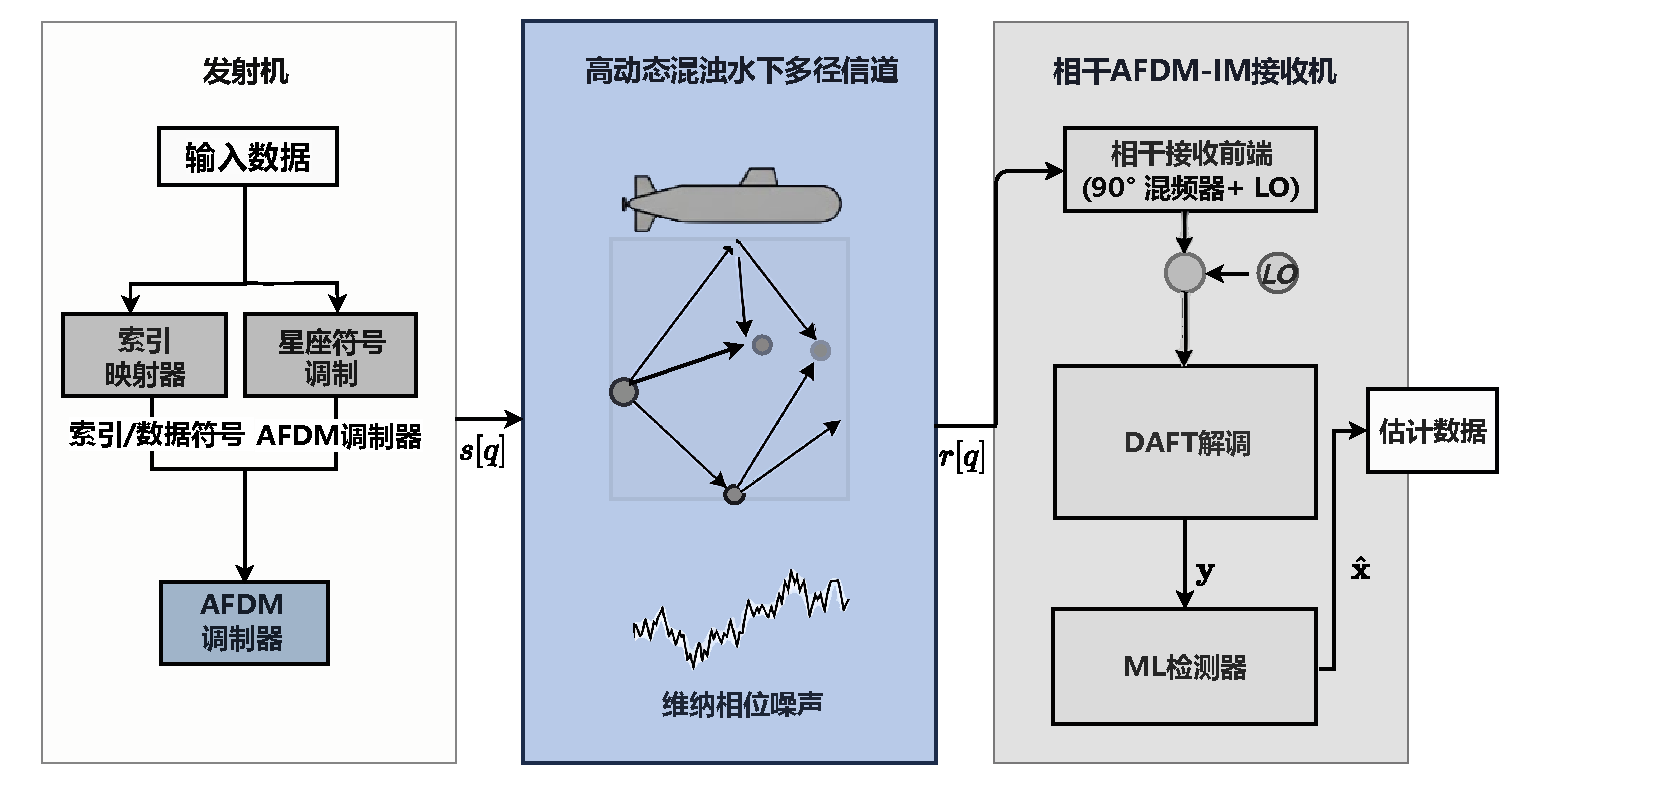
\includegraphics[width=0.85\linewidth]{figures/fig5_coherent_system.pdf}
    \caption{相干 AFDM-IM 系统完整框图}
    \label{fig:coherent_afdm_im_system}
\end{figure}

在系统整体设计上，本文将 AFDM 波形、相干接收和索引调制结构联合考虑。其基本思路是：在发射端利用 AFDM 的啁啾基构造提高系统对双选择性信道的适应能力，在符号层面通过索引调制机制引入块稀疏结构，以兼顾信息承载效率和检测复杂度；在接收端则借助相干探测恢复复数基带信号，并在 DAFT 域下建立统一的等效输入输出关系。通过这种联合设计，系统不仅能够适配高动态场景下的时延与多普勒耦合特征，还能为后续检测方法提供模型基础。

\subsection{发射端 AFDM-IM 信号构造}
\label{subsec:coherent_afdm_im_tx}

设系统总 DAFT 域维度为 $N$，将其划分为 $G$ 个等长子块，则每个子块长度为 $n=N/G$。对于第 $g$ 个子块，输入比特分为索引比特与星座比特两部分。若每个子块中有 $k$ 个激活位置，则索引比特数与星座比特数分别为
\begin{equation}
    b_{\mathrm{I}} = \left\lfloor \log_2 \binom{n}{k} \right\rfloor,
    \qquad
    b_{\mathrm{S}} = k \log_2 M
    \label{eq:im_bits_mapping}
\end{equation}
其中，$M$ 为复星座调制阶数。因此，每个子块承载的总比特数为 $b_g=b_{\mathrm{I}}+b_{\mathrm{S}}$。

上述分块设计的意义在于在频谱效率、结构稀疏性与检测复杂度之间取得平衡。若直接在整个长度为 $N$ 的向量上进行全局索引映射，虽然能够获得更大的激活模式集合，但接收端的候选搜索空间也会迅速膨胀；而将发送向量划分为多个等长子块后，可在保持较高比特承载能力的同时，将检测问题限制在局部维度上。参数 $n$、$k$ 与 $G$ 的选取因此具有明确物理意义：$n$ 决定单个子块的判决维度，$k$ 反映每个子块的激活稀疏程度，$G$ 则决定整帧中并行信息单元的数量。三者共同影响系统频谱效率、误码性能以及接收端复杂度。

记第 $g$ 个子块的 AFDM-IM 向量为 $\mathbf{x}_g \in \mathbb{C}^{n\times 1}$。其非零位置由索引集合 $\mathcal{I}_g$ 确定，其中
\begin{equation}
    \mathcal{I}_g=\{i_{g,1},i_{g,2},\ldots,i_{g,k}\}
\end{equation}
于是
\begin{equation}
    x_g[m] =
    \begin{cases}
        s_{g,u}, & m = i_{g,u},\; u=1,2,\ldots,k \\
        0, & m \notin \mathcal{I}_g
    \end{cases}
    \label{eq:subblock_im_vector}
\end{equation}
其中，$s_{g,u}\in\mathcal{S}$，$\mathcal{S}$ 表示 $M$ 阶复星座集合。将全部子块顺序拼接，可得到整帧 DAFT 域发送向量
\begin{equation}
    \mathbf{x} = [\mathbf{x}_1^T,\mathbf{x}_2^T,\ldots,\mathbf{x}_G^T]^T \in \mathbb{C}^{N\times 1}
    \label{eq:global_im_vector}
\end{equation}
其满足块稀疏约束 $\|\mathbf{x}_g\|_0=k$。

由上述结构可见，AFDM-IM 的信息承载由两部分共同组成：一部分由激活位置决定，对应索引比特；另一部分由激活位置上的复星座符号决定，对应星座比特。这种联合映射方式使系统在单位资源下可传输的信息量超过单纯依赖星座点的常规调制方式。同时，由于非激活位置保持为零，发送向量天然具有块稀疏特征，这也为后续最大似然检测提供了结构基础。图~\ref{fig:sim_bit_mapping_structure} 从比特分流与子块激活结构两个角度，对 AFDM-IM 的发送向量构造过程进行了直观说明。

\begin{figure}[htbp]
    \centering
    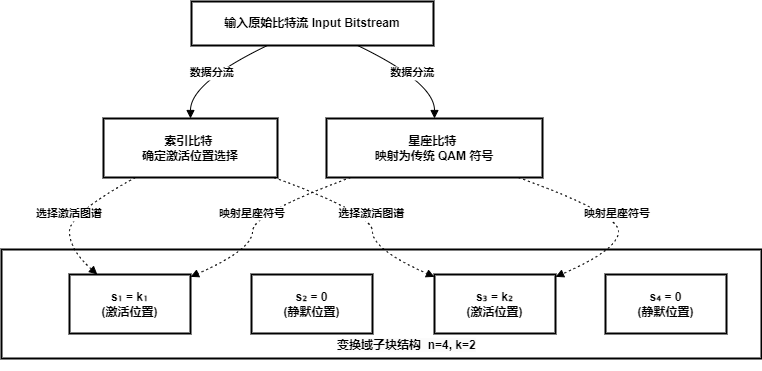
\includegraphics[width=0.82\linewidth]{figures/fig4_1_sim_bit_mapping_structure.png.png}
    \caption{AFDM-IM 子块比特映射与静默位置结构示意图}
    \label{fig:sim_bit_mapping_structure}
\end{figure}

\subsubsection{AFDM-IM 频谱效率分析}

为定量衡量所提 AFDM-IM 方案的信息承载能力，本节对其频谱效率进行分析，并与常规 AFDM（不采用索引调制）和传统 OFDM-IM 进行对比。

对于 AFDM-IM，系统每帧承载的总比特数为
\begin{equation}
    B_{\mathrm{AFDM\text{-}IM}} = G \cdot \left(\left\lfloor \log_2 \binom{n}{k} \right\rfloor + k\log_2 M\right)
    \label{eq:afdm_im_total_bits}
\end{equation}
而对于不采用索引调制的常规 AFDM，全部 $N$ 个 DAFT 域位置均加载星座符号，每帧承载比特数为
\begin{equation}
    B_{\mathrm{AFDM}} = N \log_2 M
    \label{eq:afdm_total_bits}
\end{equation}

以本章仿真参数为例（$N=256$，$G=32$，$n=8$，$k=2$，$M=4$），代入式(\ref{eq:afdm_im_total_bits}) 可得
\begin{equation}
    B_{\mathrm{AFDM\text{-}IM}} = 32 \times \left(\lfloor\log_2 28\rfloor + 2\times 2\right) = 32 \times (4+4) = 256 \text{ bit/帧}
\end{equation}
对应的归一化频谱效率为 $\eta_{\mathrm{AFDM\text{-}IM}} = 256/(256+L_{\mathrm{cp}}) \approx 0.96$ bit/s/Hz（取 $L_{\mathrm{cp}}=10$）。作为对比，常规 AFDM 的每帧比特数为 $B_{\mathrm{AFDM}} = 256 \times 2 = 512$ bit/帧，频谱效率约为 1.92 bit/s/Hz。

从上述数值可以看出，AFDM-IM 的频谱效率约为常规 AFDM 的 50\%。然而，这一对比并不构成 AFDM-IM 的劣势，原因在于：索引调制以降低绝对频谱效率为代价，换取了以下三方面收益。一是接收端检测可靠性的提升——由于每个子块仅有 $k$ 个激活位置，ML 检测的候选空间从 $M^n$ 压缩为 $\binom{n}{k}M^k$，搜索范围显著缩小，判决可靠性在有限信噪比下得以改善。二是发射信号平均功率的降低——在每个子块的 $n$ 个位置中仅 $k$ 个承载非零符号，在总能量约束下单个激活位置可分配到更高的瞬时功率，从而提高单符号信噪比。三是静默位置为接收端提供了可利用的结构先验——这正是本章后续基于静默位置泄露能量最小化方法的物理基础。

与传统 OFDM-IM 相比，AFDM-IM 在相同子块划分和激活参数下具有相同的索引比特数 $b_{\mathrm{I}}$ 和星座比特数 $b_{\mathrm{S}}$，因此两者的频谱效率完全相同。二者的性能差异完全来源于波形结构层面：AFDM 的啁啾映射使系统在高动态双选择性信道下保持更好的结构稳定性，而 OFDM 在同等多普勒条件下会因子载波正交性破坏导致严重的 ICI。进一步地，不同子块映射模式 $(n,k)$ 还会影响索引效率、平均激活能量和检测鲁棒性之间的权衡。图~\ref{fig:sim_subblock_modes} 给出了若干典型映射模式下的 BER 对比结果，可用于说明本章后续仿真中采用固定子块结构的设计依据。

\begin{figure}[htbp]
    \centering
    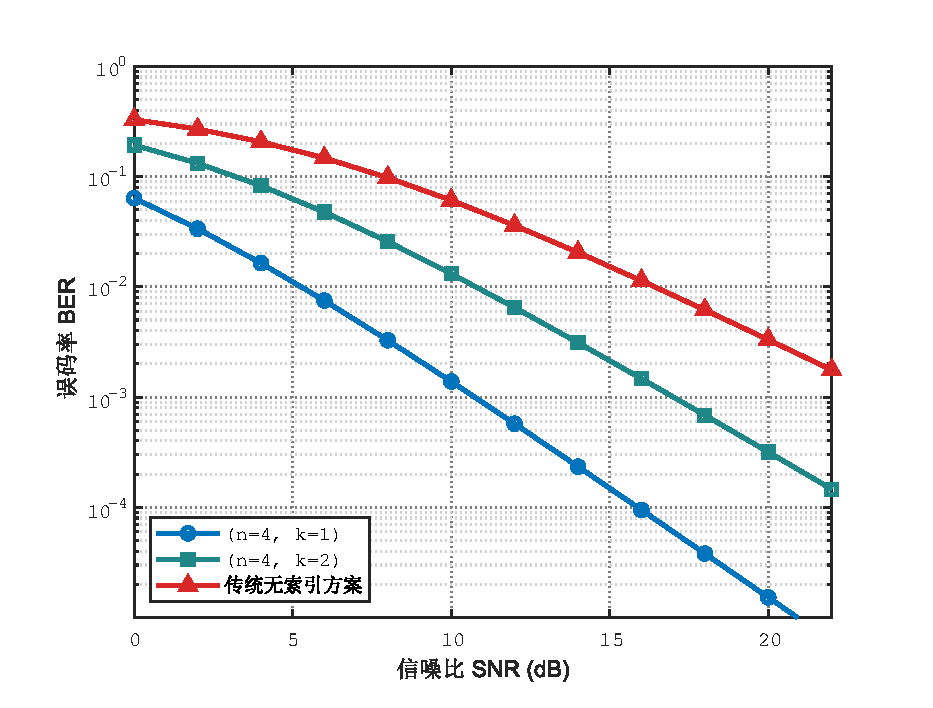
\includegraphics[width=0.85\linewidth]{figures/fig4_4_ber_sim_subblock_modes.eps}
    \caption{不同子块映射模式 $(n,k)$ 下相干 AFDM-IM 系统的 BER 性能对比}
    \label{fig:sim_subblock_modes}
\end{figure}

发送向量经离散逆仿射傅里叶变换映射至时域。记 AFDM 调制矩阵为
\begin{equation}
    \boldsymbol{\Psi} = \boldsymbol{\Lambda}_{c_1}^{H} \mathbf{F}^{H} \boldsymbol{\Lambda}_{c_2}^{H}
    \label{eq:afdm_mod_matrix}
\end{equation}
其中，$\mathbf{F}$ 为归一化 DFT 矩阵，$\boldsymbol{\Lambda}_{c_1}$ 与 $\boldsymbol{\Lambda}_{c_2}$ 分别为由啁啾参数 $c_1$ 和 $c_2$ 决定的对角相位矩阵。则离散时域基带信号为
\begin{equation}
    \mathbf{s} = \boldsymbol{\Psi}\mathbf{x}
    \label{eq:tx_signal_vector}
\end{equation}
为抑制多径引起的块间干扰，在每个 AFDM 符号前添加长度为 $L_{\mathrm{cp}}$ 的循环前缀。由于采用相干架构，发送端可直接加载复数包络信号，因此无需进行厄米特对称映射与非负限幅处理。

相较于 IM-DD 架构下对实值非负性的严格约束，相干架构允许发送端直接处理复数域波形，因此 AFDM 的复数调制优势能够得到更充分体现。另一方面，循环前缀的引入使系统在面对有限时延扩展时仍可维持较稳定的块处理结构，为后续在 DAFT 域中建立等效输入输出关系提供了前提。由此可见，AFDM-IM 发射端并不是对 AFDM 和索引调制的简单叠加，而是在高动态相干场景下对波形、映射和接收架构进行联合适配的结果。

\subsection{高动态水下相干光信道模型}
\label{subsec:coherent_afdm_im_channel}

考虑收发平台之间存在高速相对运动的高动态 UWOC 场景，信道可建模为具有 $P$ 条离散路径的线性时变系统。第 $p$ 条路径的复增益、离散时延和归一化多普勒频移分别记为 $h_p$、$l_p$ 和 $\alpha_p$。在去除循环前缀后，时域接收信号可表示为
\begin{equation}
    r[q] = e^{j\phi[q]} \sum_{p=1}^{P} h_p e^{j\frac{2\pi}{N}\alpha_p q} s[(q-l_p)_N] + w[q],
    \qquad q=0,1,\ldots,N-1
    \label{eq:time_domain_received_signal}
\end{equation}
其中，$w[q]$ 为零均值复高斯白噪声，$(\cdot)_N$ 表示模 $N$ 运算，$\phi[q]$ 表示由发射激光器与本振激光器有限线宽共同引起的离散相位噪声过程。由式(\ref{eq:time_domain_received_signal}) 可见，时域接收信号同时受到多径时延、多普勒旋转与相位噪声扰动的共同影响。

式(\ref{eq:time_domain_received_signal}) 中各参数具有明确的物理含义。$h_p$ 反映第 $p$ 条路径的复增益，既包含路径损耗信息，也包含由传播过程引起的相位变化；$l_p$ 描述离散时延，用于刻画不同路径的到达时间差；$\alpha_p$ 则表征归一化多普勒频移，用以描述相对运动导致的频率扩展效应。在高动态场景下，多个路径往往同时具有不同的时延与多普勒偏移，因此接收信号并非简单的时移叠加，而是带有时移--频移耦合特征的复合过程。

与低动态场景相比，高动态 UWOC 所面临的困难在于信道失真不再局限于静态多径扩展，而是表现为多径 + 多普勒 + 接收架构非理想的联合影响。若仅考虑多径效应，系统可通过前缀保护、变换域均衡等手段进行处理；但当多普勒扩展与器件相位不稳定性同时存在时，接收信号会出现更明显的能量扩散、星座旋转与等效信道失配，进而提高检测难度。因此，建立兼顾多径、多普勒和相位噪声的统一信道模型，对于后续算法设计具有基础性意义。

根据维纳相位噪声模型，离散相位过程满足
\begin{equation}
    \phi[q] = \phi[q-1] + \Delta[q],
    \qquad
    \Delta[q] \sim \mathcal{N}(0,\sigma_{\phi}^{2})
    \label{eq:phase_noise_process}
\end{equation}
其中，$\Delta[q]$ 为独立高斯增量，且有
\begin{equation}
    \sigma_{\phi}^{2} = 2\pi \Delta \nu T_s
    \label{eq:phase_noise_variance}
\end{equation}
其中，$\Delta\nu$ 为组合线宽，$T_s$ 为采样间隔。由式(\ref{eq:phase_noise_variance}) 可知，相位噪声方差与组合线宽和采样间隔成正比。

维纳相位噪声模型之所以适用于本文场景，是因为相干光系统中的发射激光器与本振激光器通常具有独立的相位漂移过程，其相位误差会在离散时间上呈现逐步累积的随机游走特征。组合线宽越大，相邻采样间的相位波动越强，因而更容易在接收端引起星座旋转和检测失配。对于高阶复数调制或长帧结构而言，这种累积效应会更加突出。特别是在多普勒扩展已经破坏部分结构稳定性的前提下，相位噪声的存在会进一步加剧等效信道不确定性，使接收端难以通过简单补偿获得理想性能。

将式(\ref{eq:time_domain_received_signal}) 写为矩阵形式，可得
\begin{equation}
    \mathbf{r} = \boldsymbol{\Phi} \sum_{p=1}^{P} h_p \boldsymbol{\Lambda}(\alpha_p) \boldsymbol{\Pi}^{l_p} \mathbf{s} + \mathbf{w}
    \label{eq:matrix_received_signal}
\end{equation}
其中，$\boldsymbol{\Phi}$ 为相位噪声对角矩阵，$\boldsymbol{\Lambda}(\alpha_p)$ 为多普勒旋转矩阵，$\boldsymbol{\Pi}^{l_p}$ 为循环移位矩阵。

上述矩阵形式表明，接收信号可以看作多个时移 + 多普勒旋转算子叠加后再经相位噪声扰动得到的结果。这种表示方式为后续将系统映射到 DAFT 域提供了便利，也说明高动态 UWOC 的检测问题实质上是一个在复合时变信道下的联合估计问题，而非简单的逐位置独立判决问题。

\subsection{接收端 DAFT 域等效输入输出关系}
\label{subsec:coherent_afdm_im_rx}

在接收端，去除循环前缀后的接收向量 $\mathbf{r}$ 经 AFDM 解调矩阵
\begin{equation}
    \boldsymbol{\Psi}^{H} = \boldsymbol{\Lambda}_{c_2} \mathbf{F} \boldsymbol{\Lambda}_{c_1}
    \label{eq:afdm_demod_matrix}
\end{equation}
处理后，得到 DAFT 域接收向量
\begin{equation}
    \mathbf{y} = \boldsymbol{\Psi}^{H} \mathbf{r}
    \label{eq:daft_received_signal}
\end{equation}
代入发送信号与信道模型后，可得
\begin{equation}
    \mathbf{y}
    =
    \boldsymbol{\Psi}^{H}
    \boldsymbol{\Phi}
    \sum_{p=1}^{P} h_p \boldsymbol{\Lambda}(\alpha_p) \boldsymbol{\Pi}^{l_p}
    \boldsymbol{\Psi}
    \mathbf{x}
    +
    \tilde{\mathbf{w}}
    \label{eq:equivalent_daft_io_1}
\end{equation}
其中，$\tilde{\mathbf{w}}=\boldsymbol{\Psi}^{H}\mathbf{w}$ 仍服从复高斯分布。进一步定义 DAFT 域等效信道矩阵为
\begin{equation}
    \mathbf{H}_{\mathrm{eq}}
    =
    \boldsymbol{\Psi}^{H}
    \boldsymbol{\Phi}
    \sum_{p=1}^{P} h_p \boldsymbol{\Lambda}(\alpha_p) \boldsymbol{\Pi}^{l_p}
    \boldsymbol{\Psi}
    \label{eq:equivalent_channel_matrix}
\end{equation}
则输入输出关系可统一表示为
\begin{equation}
    \mathbf{y} = \mathbf{H}_{\mathrm{eq}} \mathbf{x} + \tilde{\mathbf{w}}
    \label{eq:equivalent_daft_io_2}
\end{equation}
该式为后续检测算法推导奠定了基础，也表明检测问题可以统一表述为在等效 DAFT 域信道下对发送向量的估计问题。

\subsection{维纳相位噪声的结构化分解}
\label{subsec:phase_noise_decomposition}

式(\ref{eq:equivalent_channel_matrix}) 中的相位噪声对角矩阵 $\boldsymbol{\Phi} = \mathrm{diag}(e^{j\phi[0]}, e^{j\phi[1]}, \ldots, e^{j\phi[N-1]})$ 将维纳相位过程的逐点效应引入了等效信道表达。为后续算法设计提供理论支撑，有必要对符号周期内的维纳相位过程进行结构化分解，明确其各分量对检测性能的影响机理。

将维纳相位过程 $\phi[q]$（$q = 0, 1, \ldots, N-1$）在一个符号周期内进行正交分解：
\begin{equation}
    \phi[q] = \underbrace{\phi[0]}_{\text{常数相位}} + \underbrace{\frac{q}{N}\left(\phi[N-1]-\phi[0]\right)}_{\text{线性漂移}} + \underbrace{\epsilon[q]}_{\text{高阶随机残差}}
    \label{eq:phase_noise_decomposition}
\end{equation}
其中，三个分量具有不同的物理含义与对检测的影响方式。

常数相位分量 $\phi[0]$ 对整个符号块施加统一的相位旋转。由于最大似然检测中对发送向量的判决基于欧氏距离度量，而常数相位旋转等价于对接收信号向量进行全局旋转，不改变各候选向量与接收观测之间的距离排序，因此该分量对检测结果透明，无需显式补偿。

线性漂移分量 $\frac{q}{N}(\phi[N-1]-\phi[0])$ 在时域上表现为线性相位斜坡，其效果等价于一个小量的频率偏移。设线性漂移对应的等效归一化频偏为
\begin{equation}
    \Delta f_{\mathrm{drift}} = \frac{\phi[N-1]-\phi[0]}{2\pi}
    \label{eq:linear_drift_freq}
\end{equation}
由于 $\phi[N-1]-\phi[0] = \sum_{q=1}^{N-1}\Delta[q]$ 是 $N-1$ 个独立高斯增量的累加，其方差为 $(N-1)\sigma_\phi^2$。在典型参数条件下（$N=256$，$\Delta\nu T_s = 10^{-4}$），线性漂移分量的标准差约为 $\sqrt{(N-1) \cdot 2\pi \cdot 10^{-4}} \approx 0.40$ rad，对应的等效归一化频偏约为 $0.40/(2\pi) \approx 0.064$。该分量在形式上与残余 CFO 完全相同（均表现为时域线性相位），因此可被后续盲搜算法在搜索过程中自动吸收——算法所估计的"最优频偏补偿参数"实际上是真实 CFO 与线性漂移之和，二者无需分别处理。

高阶随机残差 $\epsilon[q]$ 是维纳相位过程去除常数和线性分量后的剩余部分，表现为零均值、时间相关的随机波动。其方差可通过布朗桥模型给出上界：
\begin{equation}
    \mathrm{Var}[\epsilon[q]] \leq \frac{q(N-1-q)}{N-1} \sigma_\phi^2
    \label{eq:residual_variance_bound}
\end{equation}
该上界在 $q = (N-1)/2$ 处取得最大值 $(N-1)\sigma_\phi^2/4$。在本文典型参数下，$\max_q \mathrm{Var}[\epsilon[q]] \approx 255 \times 2\pi \times 10^{-4}/4 \approx 0.040$ rad$^2$，对应的标准差约为 0.20 rad。

当残差相位较小时（$|\epsilon[q]| \ll 1$），可对相位噪声指数进行线性化近似：
\begin{equation}
    e^{j\epsilon[q]} \approx 1 + j\epsilon[q]
    \label{eq:phase_noise_linearization}
\end{equation}
该近似的有效条件为 $\mathrm{Var}[\epsilon[q]] \ll 1$ rad$^2$。在本文仿真条件下，最大残差方差为 0.040 rad$^2$，远小于 1，因此线性化近似成立。此时，高阶随机残差的效果等价于在接收信号上叠加一个功率受限的附加噪声项：
\begin{equation}
    e^{j\epsilon[q]} \cdot r_{\mathrm{comp}}[q] \approx r_{\mathrm{comp}}[q] + j\epsilon[q] \cdot r_{\mathrm{comp}}[q]
    \label{eq:residual_as_noise}
\end{equation}
其中 $r_{\mathrm{comp}}[q]$ 为经 CFO 补偿后的接收信号。第二项可视为信号依赖型附加噪声，其功率与信号功率和残差方差的乘积成正比。

上述分解的意义在于：维纳相位噪声中对检测性能影响最大的两个分量（常数相位和线性漂移）恰好分别被 ML 检测的距离度量不变性和盲搜算法的频偏吸收能力自动处理，而剩余的高阶随机残差在线性化近似下等效为功率受限的附加噪声。这一分析为后续将维纳相位噪声作为等效背景干扰纳入残余噪声项处理提供了严格的理论依据，也解释了为何所提算法能够在不显式估计完整维纳相位过程的情况下仍对相位噪声保持鲁棒容忍。

\subsection{DAFT 域等效信道矩阵的结构特性}
\label{subsec:daft_channel_structure}

为深入理解 AFDM 在高动态场景中的性能优势来源，本节对式(\ref{eq:equivalent_channel_matrix}) 所定义的 DAFT 域等效信道矩阵 $\mathbf{H}_{\mathrm{eq}}$ 的结构特性进行分析。

在不考虑相位噪声的理想条件下（即 $\boldsymbol{\Phi} = \mathbf{I}$），等效信道矩阵退化为
\begin{equation}
    \mathbf{H}_{\mathrm{eq}}^{(\mathrm{ideal})} = \boldsymbol{\Psi}^{H} \sum_{p=1}^{P} h_p \boldsymbol{\Lambda}(\alpha_p) \boldsymbol{\Pi}^{l_p} \boldsymbol{\Psi}
    \label{eq:ideal_equiv_channel}
\end{equation}

对于单条路径（$P=1$，$h_1=1$，$l_1=l$，$\alpha_1=\alpha$），利用 DAFT 调制矩阵的解析形式，可将等效信道矩阵的第 $(m,k)$ 元素表示为
\begin{equation}
    [\mathbf{H}_{\mathrm{eq}}^{(\mathrm{ideal})}]_{m,k} = h_1 \cdot \delta\!\left[(m - k - 2Nc_1 l - 2Nc_2\alpha)_N\right] \cdot e^{j\varphi_{m,k}}
    \label{eq:single_path_channel_element}
\end{equation}
其中 $\varphi_{m,k}$ 为与啁啾参数和路径参数相关的相位项，$\delta[\cdot]$ 为克罗内克 delta 函数。式(\ref{eq:single_path_channel_element}) 表明，单条路径在 DAFT 域中对应等效信道矩阵的一条对角线（偏移量为 $(2Nc_1 l + 2Nc_2\alpha)_N$）。

当存在多条路径时，等效信道矩阵为各路径贡献的叠加：
\begin{equation}
    \mathbf{H}_{\mathrm{eq}}^{(\mathrm{ideal})} = \sum_{p=1}^{P} h_p \cdot \mathbf{D}_p
    \label{eq:multipath_channel_superposition}
\end{equation}
其中 $\mathbf{D}_p$ 为第 $p$ 条路径对应的移位对角矩阵，其非零元素位于第 $(2Nc_1 l_p + 2Nc_2\alpha_p)_N$ 条对角线上。该结构具有以下重要性质。

当啁啾参数 $c_1$ 和 $c_2$ 设计合理时，不同路径对应的对角线偏移量相互区分，使等效信道矩阵呈现稀疏的多对角线结构。在这种条件下，DAFT 域中每个接收位置仅与有限个发送位置耦合，检测算法可利用这种稀疏性降低计算复杂度。当路径的时延-多普勒参数对满足分离条件
\begin{equation}
    (2Nc_1 l_p + 2Nc_2\alpha_p)_N \neq (2Nc_1 l_q + 2Nc_2\alpha_q)_N, \quad \forall p \neq q
    \label{eq:path_separation_condition_ch4}
\end{equation}
时，各路径在 DAFT 域中占据不同的对角线位置，接收端可通过结构化检测联合利用所有路径能量，获得满分集增益。

与 OFDM 的等效信道矩阵进行对比可进一步揭示 AFDM 的优势。对于 OFDM 系统，在无多普勒条件下，等效信道为对角矩阵，各子载波独立经历频率选择性衰落；当存在多普勒时，等效信道变为满矩阵（非稀疏），每个接收位置与所有发送位置耦合，产生全局性的 ICI。AFDM 则通过啁啾参数的引入，将时延-多普勒耦合映射为 DAFT 域中的确定性位置偏移，使等效信道在双选择性条件下仍保持稀疏结构，这正是其抗多普勒能力优于 OFDM 的根本原因。

\section{基于静默位置泄露能量最小化的残余 CFO 补偿与检测方法}
\label{sec:silent_leakage_phase_comp}

在上一节的系统模型中，时域接收信号同时受到多径时延、多普勒频移以及维纳相位噪声的联合影响。在高动态 UWOC 场景下，上述因素中对 DAFT 域子载波正交性破坏最为严重的是多普勒效应所引发的载波频率偏移（Carrier Frequency Offset, CFO）。载波频偏在时域表现为线性相位斜坡，经 DAFT 变换后会导致能量从激活位置大规模扩散至相邻位置，从而使原本应为零的静默位置上出现显著的残余能量——这正是静默位置泄露的核心物理来源。相比之下，维纳相位噪声虽然也会引起逐点时变的相位扰动，但其随机游走特性使其在单符号尺度上的主要效应表现为叠加在残余频偏之上的随机结构扰动，而非可由单一标量直接表征并完全补偿的确定性泄露来源。

基于上述物理认识，本节进一步利用 AFDM-IM 发送向量的块稀疏结构，构造一种基于静默位置泄露能量最小化的盲/半盲残余 CFO 补偿与检测方法。该方法不再将索引调制仅视为频谱效率增强手段，而是进一步把未激活位置所蕴含的零结构先验转化为接收端可利用的隐式参考信息，从而在减少或避免显式导频开销的前提下完成主导残余频偏分量的感知、补偿与后续检测。

本节将待估参数建模为归一化残余频率偏移 $\theta$，其物理意义对应于多普勒效应在接收端引起的等效载波频偏。由于维纳相位噪声是逐点时变的随机过程，无法被单一标量参数完全描述或消除，本文的算法框架将其视为等效背景干扰，与热噪声一并纳入残余噪声项处理。这一建模选择的合理性将通过后续仿真得到验证：算法能够精准补偿主导频偏分量，使系统 BER 显著优于传统导频方案；而由于残余维纳相位噪声的存在，系统相较于理想下界保留极小的性能折损，体现了工程上的合理鲁棒性。

\subsection{基本思想与问题建模}
\label{subsec:silent_leakage_principle}

对于第 $g$ 个子块，AFDM-IM 发送向量 $\mathbf{x}_g\in\mathbb{C}^{n\times 1}$ 满足稀疏激活约束 $\|\mathbf{x}_g\|_0=k<n$。若记其激活位置集合为 $\mathcal{I}_g$，则静默位置集合可写为 $\mathcal{Z}_g=\{1,2,\ldots,n\}\setminus\mathcal{I}_g$。理想情况下，对于任意 $m\in\mathcal{Z}_g$，均有
\begin{equation}
    x_g[m]=0.
\end{equation}
在无频偏且无相位噪声时，DAFT 域接收信号的能量将严格集中在激活位置上，静默位置保持为零。然而，当存在多普勒效应引起的载波频偏时，时域信号相当于被乘以线性相位斜坡 $e^{j2\pi\theta q/N}$（其中 $\theta$ 为归一化频偏参数），该线性相位在经过 DAFT 变换后会破坏子载波间的正交性，导致能量从激活位置向相邻位置大规模扩散，从而在静默位置上产生显著的残余分量。这种由频偏引起的载波间干扰（ICI）和能量泄露，正是静默位置泄露能量最小化准则所针对的核心失真。

为明确区分不同失真机制对能量泄露的贡献，可对接收端观测到的静默位置残余能量做如下定性分析。一方面，若仅存在恒定相位偏移 $e^{j\phi_0}$（即常数相位旋转），由于酉变换的保模性质，DAFT 域各位置的能量分布不会改变，静默位置仍为零——因此，纯常数相位不会引起能量泄露，也无法通过静默位置能量准则加以估计。另一方面，线性相位斜坡（即载波频偏）会在变换域引起系统性的子载波间能量扩散，其效应随频偏增大而显著增强，是能量泄露的主导来源。至于维纳相位噪声，由于其为逐采样点独立累积的随机游走过程，无法被任何单一标量参数所完整描述，其效应在本文算法框架中被归入等效残余干扰处理。

基于上述分析，本文将待估参数 $\theta$ 明确定义为归一化残余载波频偏。在高动态 UWOC 场景中，该参数主要源自收发平台相对运动所导致的多普勒频移。定义频偏补偿矩阵为
\begin{equation}
    \boldsymbol{\Phi}(\theta) = \mathrm{diag}\left(1,\, e^{j2\pi\theta/N},\, \ldots,\, e^{j2\pi\theta(N-1)/N}\right)
    \label{eq:cfo_compensation_matrix}
\end{equation}
该矩阵作用在时域接收向量上可消除频偏所引起的线性相位斜坡。对第 $g$ 个子块，经频偏补偿后的 DAFT 域观测向量为
\begin{equation}
    \mathbf{z}_g(\theta) = \boldsymbol{\Psi}^{H}\boldsymbol{\Phi}^{H}(\theta)\mathbf{r}_g
    \label{eq:compensated_observation}
\end{equation}
其中 $\boldsymbol{\Psi}^{H}$ 为 AFDM 解调矩阵。若频偏参数补偿正确，线性相位斜坡被消除后，DAFT 域的正交性得到恢复，能量将重新集中于激活位置，静默位置的残余能量降至最低。据此，可构造如下静默位置泄露能量最小化准则：
\begin{equation}
    \hat{\theta}=\arg\min_{\theta}
    \sum_{g=1}^{G}\sum_{m\in\mathcal{Z}_g}
    \left|z_g^{(m)}(\theta)\right|^2.
    \label{eq:silent_energy_direct}
\end{equation}
式(\ref{eq:silent_energy_direct}) 的物理含义明确：在候选频偏参数空间中搜索使静默位置残余能量最小的补偿值，即为对主导多普勒频偏的最优估计。当补偿值 $\theta$ 接近真实频偏时，被频偏推散到静默位置的能量将被最大程度地压缩回激活位置。图~\ref{fig:residual_cfo_sensitivity} 进一步给出了系统 BER 随残余 CFO 失配程度变化的趋势，可以看到即便在固定 SNR 条件下，若不对主导残余频偏进行有效补偿，误码性能也会迅速恶化，这正是后续盲补偿算法必须解决的核心问题。

\begin{figure}[htbp]
    \centering
    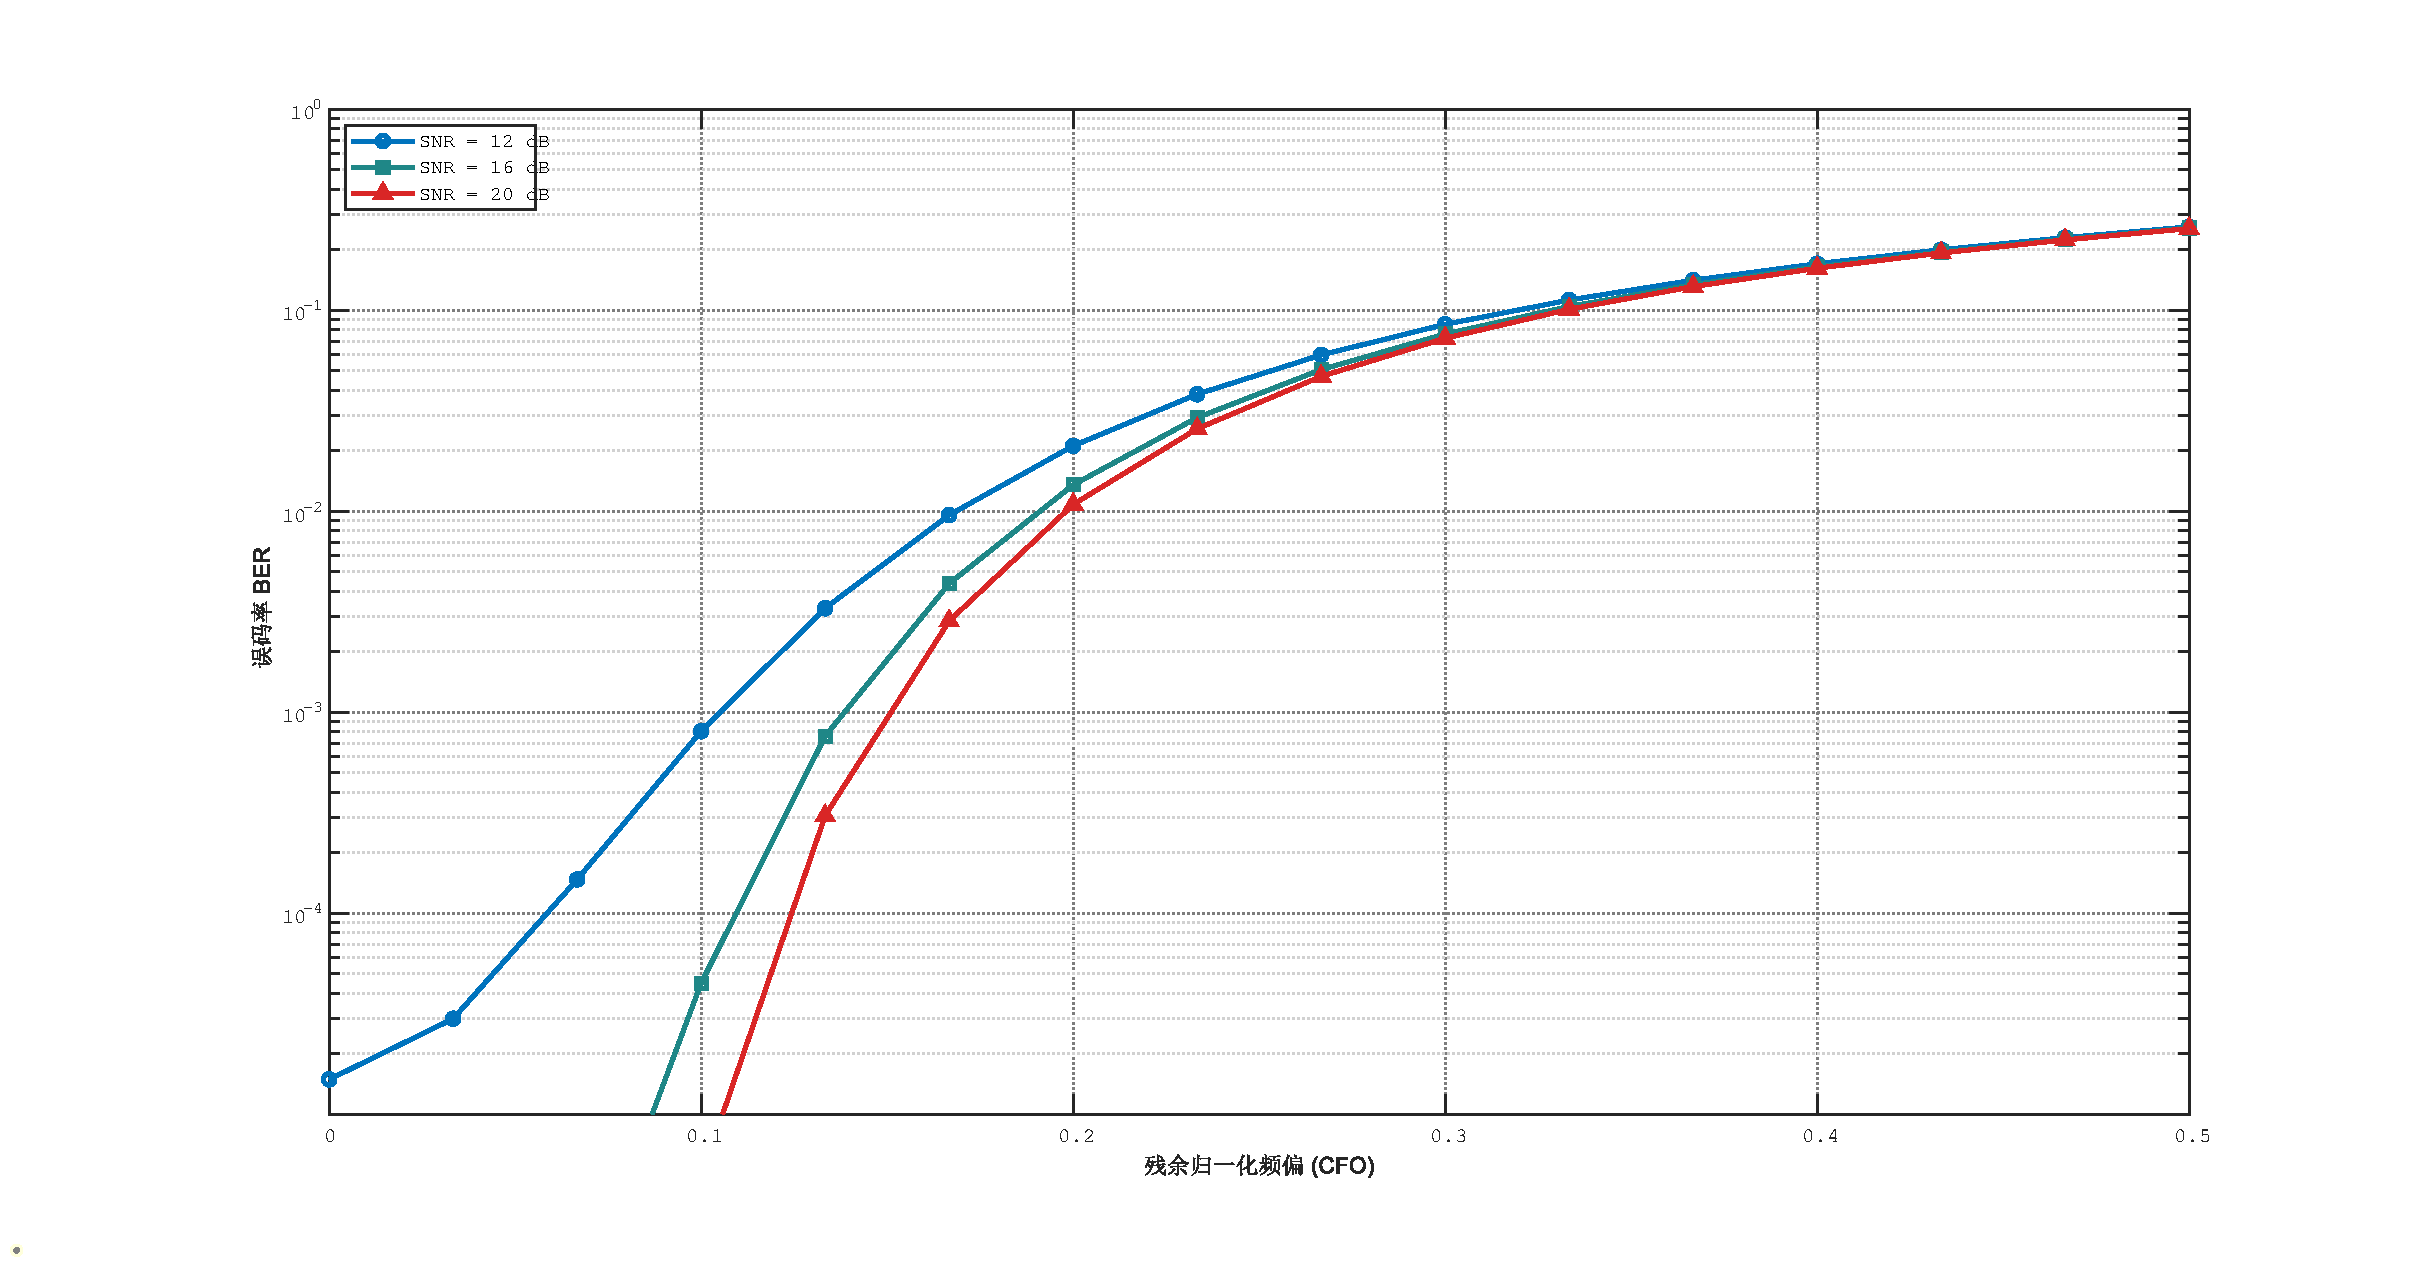
\includegraphics[width=0.85\linewidth]{figures/fig4_3_ber_residual_cfo_sensitivity.eps}
    \caption{不同残余 CFO 失配程度下相干 AFDM-IM 系统的 BER 敏感性曲线}
    \label{fig:residual_cfo_sensitivity}
\end{figure}

维纳相位噪声作为叠加在频偏之上的逐点随机扰动，会在补偿后引入无法被单一参数 $\theta$ 消除的残余干扰。然而，在典型系统配置下（$N=256$，中等组合线宽），单符号内的维纳累积相位方差 $N\sigma_\phi^2 = 2\pi\Delta\nu T_{\mathrm{sym}}$ 仍保持在较小水平，其引起的附加能量泄露远弱于未补偿频偏的贡献。因此，所提准则在实际工作条件下仍能有效捕获主导频偏分量，使系统 BER 显著优于传统方案。残余维纳相位噪声的影响则体现为系统相对于理想下界存在极小的性能折损，这一现象将在仿真分析中得到进一步验证。

为进一步从理论层面支撑维纳相位噪声可近似视为等效背景干扰这一建模假设，下面对单个 AFDM 符号周期内的离散相位噪声过程进行结构化分解。根据式(\ref{eq:phase_noise_process})，维纳相位过程 $\phi[q]$（$q=0,1,\ldots,N-1$）是零起点随机游走的累积和。对 $\phi[q]$ 在符号周期内进行最小二乘线性拟合，可将其分解为三个正交分量：
\begin{equation}
    \phi[q] = \underbrace{\bar{\phi}}_{\text{常数相位}} + \underbrace{2\pi f_{\mathrm{drift}} \cdot q T_s}_{\text{线性漂移（等效频偏）}} + \underbrace{\epsilon[q]}_{\text{高阶随机残差}}
    \label{eq:phase_noise_decomposition_ls}
\end{equation}
其中，$\bar{\phi}=\frac{1}{N}\sum_{q=0}^{N-1}\phi[q]$ 为符号内平均相位；$f_{\mathrm{drift}}$ 为通过最小二乘拟合得到的等效线性频率漂移率；$\epsilon[q]$ 为去除常数项与线性趋势后的残余高阶随机分量。

式(\ref{eq:phase_noise_decomposition_ls}) 中三个分量对 DAFT 域静默位置能量泄露的贡献截然不同。第一项 $\bar{\phi}$ 为常数相位旋转，由前述分析可知，酉变换的保模性质使其不改变 DAFT 域的能量分布，因此不会引起静默位置泄露，对本文盲搜准则透明。第二项为线性相位斜坡，其效应等价于一个附加的归一化频偏 $\theta_{\mathrm{drift}}=f_{\mathrm{drift}} N T_s$，会引起系统性的子载波间能量扩散；然而，该分量在本文算法中会被自动吸收到待估频偏参数 $\theta$ 中，即盲搜过程实际估计的是多普勒 CFO + 维纳线性漂移的合成频偏，因此不会造成额外的性能损失。第三项 $\epsilon[q]$ 才是真正无法被单一标量参数所描述或消除的残余随机分量，其统计特性决定了维纳相位噪声作为等效背景干扰的强度上界。

对残差项 $\epsilon[q]$ 的统计特性，可通过如下方式给出定量界限。由于 $\phi[q]$ 的增量 $\Delta[q]$ 为独立同分布高斯变量（方差 $\sigma_\phi^2 = 2\pi\Delta\nu T_s$），经过线性去趋势后的残差方差可以表示为
\begin{equation}
    \mathrm{Var}[\epsilon[q]] \leq N \sigma_\phi^2 = 2\pi \Delta\nu T_{\mathrm{sym}}
    \label{eq:residual_phase_variance}
\end{equation}
其中 $T_{\mathrm{sym}}=NT_s$ 为一个 AFDM 符号的持续时间。当残差 $\epsilon[q]$ 较小时（即 $\mathrm{Var}[\epsilon[q]] \ll 1$），相位噪声对接收信号的乘性扰动 $e^{j\epsilon[q]}$ 可近似展开为
\begin{equation}
    e^{j\epsilon[q]} \approx 1 + j\epsilon[q]
    \label{eq:phase_noise_linearization_ls}
\end{equation}
代入时域接收信号模型，经 DAFT 变换后，残差相位噪声项对 DAFT 域第 $m$ 个位置的贡献可以写为
\begin{equation}
    \tilde{w}_{\phi}[m] = \sum_{q=0}^{N-1} [\boldsymbol{\Psi}^H]_{m,q} \cdot j\epsilon[q] \cdot s[q]
    \label{eq:phase_noise_interference}
\end{equation}
由于 $\epsilon[q]$ 在去趋势后近似为零均值、弱相关的随机过程，而 DAFT 变换本身具有类酉结构，因此 $\tilde{w}_{\phi}[m]$ 在统计上近似为零均值、方差正比于 $\mathrm{Var}[\epsilon[q]]$ 与信号功率乘积的附加干扰项。在中等组合线宽条件下（例如 $\Delta\nu=1\,\mathrm{MHz}$，$T_{\mathrm{sym}} \approx 10\,\mu\mathrm{s}$），有 $2\pi\Delta\nu T_{\mathrm{sym}} \approx 0.063\,\mathrm{rad}^2$，对应的相位标准差约为 $0.25\,\mathrm{rad}$（约 $14^\circ$），其引起的等效干噪比退化远小于未补偿 CFO 引起的灾难性能量泄露。

上述分析从理论上支撑了本文的建模选择：在 $2\pi\Delta\nu T_{\mathrm{sym}} \ll 1$ 的条件下，维纳相位噪声中的常数分量对检测透明，线性漂移分量被盲搜算法自动吸收，而高阶随机残差的统计效应可等效为一种功率受限的附加噪声。这意味着维纳相位噪声在本文算法框架中确实可以被合理地降维处理为等效背景干扰，而无需为其单独设计估计模块。

图~\ref{fig:constellation_comp} 以接收端星座图演化的方式，从视觉层面进一步验证了上述理论分析的正确性。

\begin{figure}[htbp]    
    \centering
    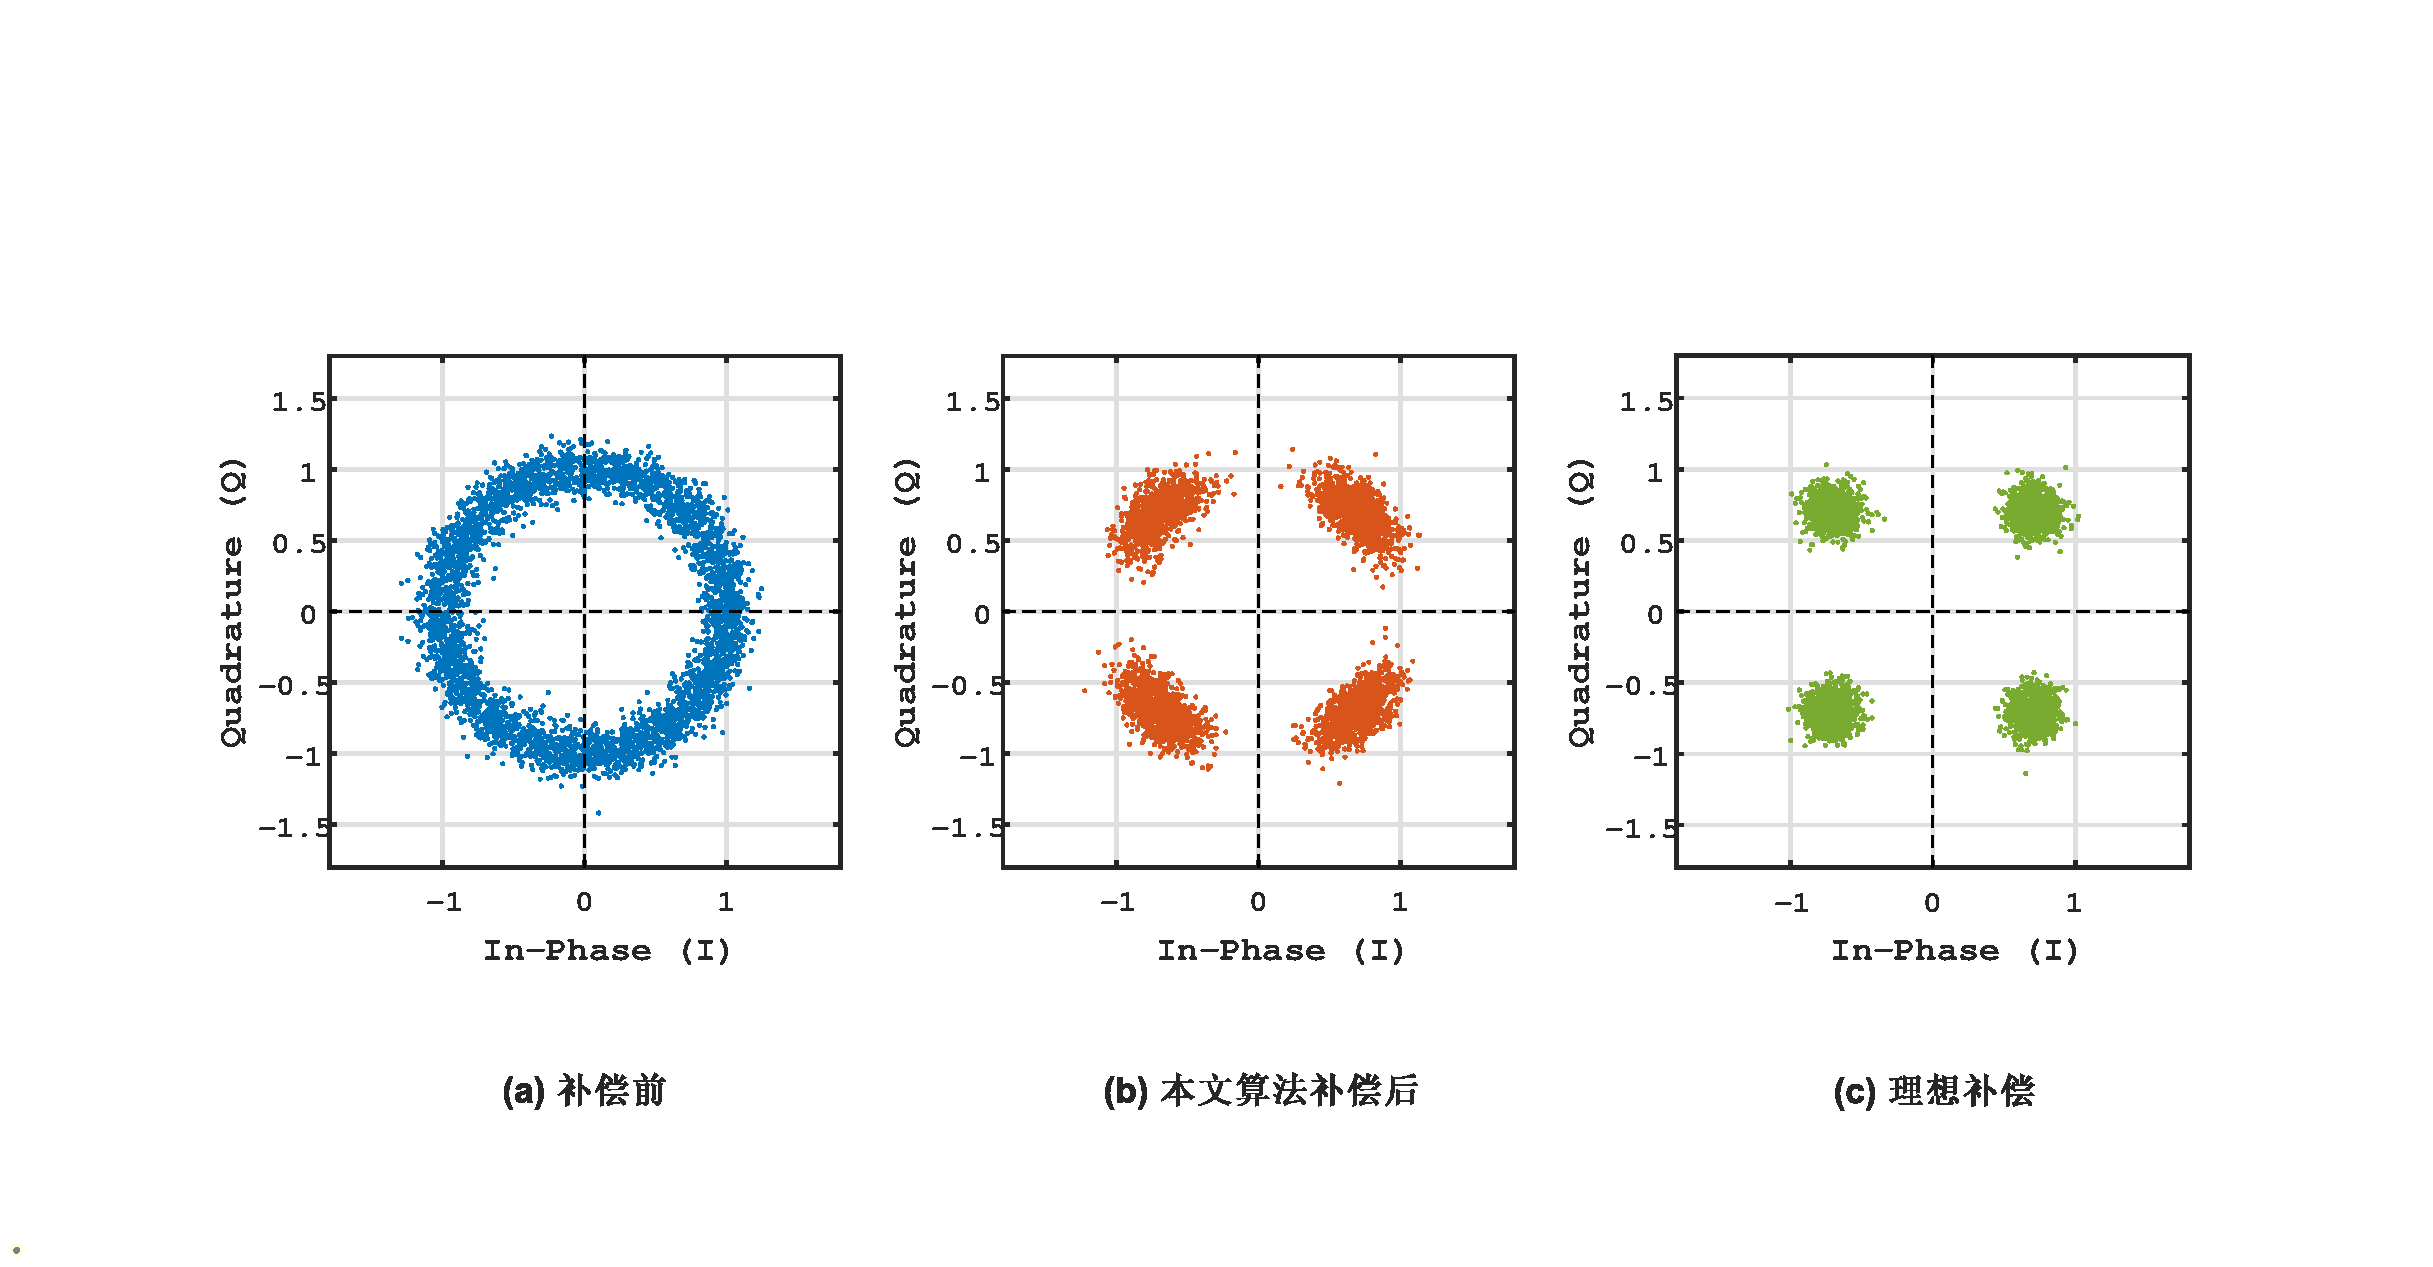
\includegraphics[width=1.0\linewidth]{figures/fig9_Constellation_Comp.eps}
    \caption{接收端星座图演化对比：(a) 补偿前；(b) 本文算法补偿后；(c) 理想补偿}
    \label{fig:constellation_comp}
\end{figure} 

由图~\ref{fig:constellation_comp}(a) 可见，在未进行任何频偏补偿时，多普勒 CFO 引起的线性相位斜坡使所有星座点沿角度方向发生完全的环状扩散，此时接收端已无法区分不同星座符号，系统处于完全失效状态。图~\ref{fig:constellation_comp}(b) 对应本文盲搜算法补偿后的结果：CFO 被精准消除，4 个星座簇重新分离，但由于残余维纳相位噪声的存在，各簇呈现出特征性的角向弧形扩散（Angular Spreading）——这正是式(\ref{eq:phase_noise_decomposition_ls}) 中高阶随机残差 $\epsilon[q]$ 的视觉表征。弧形扩散的宽度直接反映了残余相位噪声的方差大小，而其方向沿角度维度而非径向方向，说明残余扰动的主要效应是相位抖动而非幅度失真，与前述 $e^{j\epsilon[q]}\approx 1+j\epsilon[q]$ 的线性化近似完全一致。图~\ref{fig:constellation_comp}(c) 为理想补偿下的星座图，星座点呈现标准的高斯圆形模糊，仅受热噪声影响。对比 (b) 与 (c) 可以看出，本文算法补偿后的星座图与理想情形之间的差异仅为轻微的角向展宽，对应的 BER 退化极为有限，从而直观验证了将维纳相位噪声视为等效背景干扰的合理性。

此外，式(\ref{eq:silent_energy_direct}) 与传统基于导频的最小二乘频偏估计在形式上具有对偶性。传统方法通过最小化已知导频与接收观测之间的残差来估计频偏，而本文方法则通过最小化理论应为零的位置与实际观测之间的残差进行估计。二者同属于基于参考约束的参数估计框架，只是参考信息的来源不同：前者依赖显式非零导频符号，后者利用 AFDM-IM 结构天然提供的隐式零约束。

\subsection{未知索引状态下的联合估计问题}
\label{subsec:joint_estimation_unknown_index}

上述思路面临的关键困难在于：在接收端成功完成索引检测之前，静默位置集合 $\mathcal{Z}_g$ 本身是未知的，因此无法直接利用式(\ref{eq:silent_energy_direct}) 进行频偏估计。这意味着残余 CFO 估计与索引恢复之间存在显著耦合：频偏补偿不准确会影响索引检测，而索引未知又会限制静默位置残余能量准则的直接应用。

针对这一问题，可从联合最大似然角度重新建模。沿用式(\ref{eq:cfo_compensation_matrix}) 的频偏补偿模型，对第 $g$ 个子块的接收模型可写为
\begin{equation}
    \mathbf{y}_g = \boldsymbol{\Phi}(\theta)\mathbf{H}_g\mathbf{x}_g + \mathbf{w}_g
    \label{eq:joint_ml_model}
\end{equation}
其中，$\boldsymbol{\Phi}(\theta)$ 为式(\ref{eq:cfo_compensation_matrix}) 定义的频偏补偿矩阵，$\mathbf{x}_g\in\mathcal{X}_{\mathrm{IM}}$ 为满足 AFDM-IM 激活规则的候选向量集合，$\mathbf{w}_g$ 为包含热噪声与残余维纳相位噪声的等效噪声项。于是，残余 CFO 参数与发送向量的联合估计问题可写为
\begin{equation}
    (\hat{\theta},\hat{\mathbf{x}}_g)
    =
    \arg\min_{\theta,\mathbf{x}_g\in\mathcal{X}_{\mathrm{IM}}}
    \left\|\mathbf{y}_g-\boldsymbol{\Phi}(\theta)\mathbf{H}_g\mathbf{x}_g\right\|_2^2.
    \label{eq:joint_ml_theta_x}
\end{equation}
由于发送向量与激活位置集合一一对应，式(\ref{eq:joint_ml_theta_x}) 也可视为对 $(\theta,\mathcal{I}_g)$ 或 $(\theta,\mathcal{Z}_g)$ 的联合搜索。该表述说明，残余 CFO 估计并非必须先于索引检测单独完成，而是可以与索引恢复统一为一个带有结构先验的联合估计问题。

尽管式(\ref{eq:joint_ml_theta_x}) 在理论上较为完整，但若直接对残余 CFO 参数和全部合法激活模式进行穷举，其复杂度会随子块规模和调制阶数迅速上升。为此，本文进一步利用 AFDM-IM 结构的能量集中性，构造不显式依赖静默位置集合的稀疏度量，用于残余 CFO 参数的粗估计。

\subsection{基于稀疏度量的残余 CFO 粗搜索}
\label{subsec:sparsity_coarse_search}

AFDM-IM 向量在正确频偏补偿下应表现出更明显的块稀疏特征：激活位置上的有效分量更集中，而静默位置上的泄露能量更弱。相反，当残余 CFO 补偿存在失配时，能量会向非激活位置扩散，导致补偿后向量的稀疏性下降。基于这一性质，可在不预先知道 $\mathcal{Z}_g$ 的情况下，通过稀疏度量对残余 CFO 参数进行盲粗搜索。

设
\begin{equation}
    \mathbf{z}_g(\theta)=\boldsymbol{\Phi}^{H}(\theta)\mathbf{y}_g,
\end{equation}
记 $\mathcal{T}_{g,k}(\theta)$ 为 $\mathbf{z}_g(\theta)$ 中能量最大的前 $k$ 个分量索引集合，则可定义第 $g$ 个子块的能量集中度指标为
\begin{equation}
    R_{g,k}(\theta)
    =
    \frac{\sum\limits_{i\in\mathcal{T}_{g,k}(\theta)}\left|z_{g,i}(\theta)\right|^2}
    {\sum\limits_{i=1}^{n}\left|z_{g,i}(\theta)\right|^2}.
    \label{eq:block_concentration_metric}
\end{equation}
将所有子块求和或取平均后，可得到整帧残余 CFO 粗搜索指标
\begin{equation}
    R_k(\theta)
    =
    \frac{1}{G}
    \sum_{g=1}^{G}
    R_{g,k}(\theta).
    \label{eq:global_concentration_metric}
\end{equation}
于是，初始残余 CFO 估计值可由一维网格搜索得到：
\begin{equation}
    \theta^{(0)}=\arg\max_{\theta\in\Theta} R_k(\theta)
    \label{eq:coarse_theta_search}
\end{equation}
其中，$\Theta$ 为预定义的候选频偏参数集合。式(\ref{eq:coarse_theta_search}) 的含义在于：正确的频偏补偿将使补偿后信号的能量更加集中于少数主导分量，从而使 $R_k(\theta)$ 取得更大值。由于该搜索仅涉及一维频偏参数，因此在实现上具有可控的计算复杂度。

\subsection{交替优化的精细残余 CFO 补偿与检测}
\label{subsec:alternating_phase_detection}

基于稀疏度量得到的粗估计 $\theta^{(0)}$ 可作为后续联合优化的初始值。在此基础上，本文采用交替优化策略迭代更新残余 CFO 参数与发送向量估计，以降低直接联合搜索的复杂度。设第 $t$ 次迭代的残余 CFO 估计值为 $\theta^{(t)}$，则首先固定当前频偏参数，对发送向量执行分块最大似然检测：
\begin{equation}
    \hat{\mathbf{x}}_g^{(t)}
    =
    \arg\min_{\mathbf{x}_g\in\mathcal{X}_{\mathrm{IM}}}
    \left\|\mathbf{y}_g-\boldsymbol{\Phi}(\theta^{(t)})\mathbf{H}_g\mathbf{x}_g\right\|_2^2.
    \label{eq:alternating_detect_x}
\end{equation}
由式(\ref{eq:alternating_detect_x}) 得到的 $\hat{\mathbf{x}}_g^{(t)}$ 可进一步导出当前的激活位置与静默位置估计集合，分别记为 $\hat{\mathcal{I}}_g^{(t)}$ 与 $\hat{\mathcal{Z}}_g^{(t)}$。随后，固定当前发送向量估计，对残余 CFO 参数进行更新：
\begin{equation}
    \theta^{(t+1)}
    =
    \arg\min_{\theta}
    \sum_{g=1}^{G}
    \sum_{m\in\hat{\mathcal{Z}}_g^{(t)}}
    \left|\left[\boldsymbol{\Phi}^{H}(\theta)\mathbf{y}_g\right]_m\right|^2.
    \label{eq:alternating_update_theta}
\end{equation}
式(\ref{eq:alternating_update_theta}) 表明，参数更新步骤利用当前检测结果所对应的静默结构，对补偿后残余泄露能量进行再次压缩。如此反复交替，直到满足
\begin{equation}
    \left|\theta^{(t+1)}-\theta^{(t)}\right|<\varepsilon
    \quad\text{或}\quad
    t=I_{\max}
    \label{eq:alternating_stop}
\end{equation}
其中，$\varepsilon$ 为收敛阈值，$I_{\max}$ 为最大迭代次数。

该交替优化过程在形式上与 EM 类或交替最小化方法相似：一方面，通过固定残余 CFO 估计恢复更可靠的结构信息；另一方面，再利用更新后的结构信息改进频偏补偿。由于 AFDM-IM 发送向量天然具有块稀疏先验，这一迭代过程能够逐步增强主导分量与静默位置之间的分离程度，从而打破未知静默位置无法估计频偏、频偏未知又难以恢复静默位置的耦合困境。

\subsection{算法流程描述}
\label{subsec:algorithm_description}

综合上述推导，所提基于静默位置泄露能量最小化的残余 CFO 补偿与检测方法可概括为如下两阶段流程。

第一阶段为基于稀疏度量的粗搜索。接收端在候选频偏参数集合 $\Theta$ 上逐点计算补偿后信号，并依据式(\ref{eq:global_concentration_metric}) 评价其能量集中程度，随后选取使 $R_k(\theta)$ 最大的候选值作为初始残余 CFO 估计 $\theta^{(0)}$。

第二阶段为交替优化的精细补偿与检测。以 $\theta^{(0)}$ 为初始值，交替执行以下两步：其一，依据式(\ref{eq:alternating_detect_x}) 在固定频偏参数下完成 AFDM-IM 的分块最大似然检测，获得发送向量及静默位置估计；其二，依据式(\ref{eq:alternating_update_theta}) 在固定静默结构下更新残余 CFO 参数。经过有限次迭代后，输出最终残余 CFO 估计值 $\hat{\theta}$ 与发送向量估计值 $\hat{\mathbf{x}}$。

若采用算法环境表示，上述过程可表述为算法流程如下。

为便于将这一较长的接收链路与后续性能结果对应起来，表~\ref{tab:coherent_afdm_im_pipeline} 对所提相干 AFDM-IM 接收处理流程的关键步骤、功能目标及主要复杂度来源进行了总结。该表强调的是算法链路中的功能分工，而非重复公式推导。

\begin{table}[htbp]
    \centering
    \caption{相干 AFDM-IM 接收处理流程与功能说明表}
    \label{tab:coherent_afdm_im_pipeline}
    \begin{tabular}{p{1.0cm}p{2.6cm}p{2.2cm}p{3.0cm}p{2.2cm}}
        \toprule
        步骤序号 & 处理模块 & 输入/输出 & 核心功能 & 主要复杂度来源 \\
        \midrule
        1 & 前端接收与 DAFT 解调 & 时域接收信号 / DAFT 域观测向量 & 将多径、多普勒和相位扰动映射到统一的结构化表示域 & 变换运算与逐点相位补偿 \\
        2 & 稀疏度量粗搜索 & DAFT 域观测 / 初始频偏估计 $\theta^{(0)}$ & 通过能量集中度指标定位主导残余 CFO 的候选邻域 & 一维频偏网格搜索 \\
        3 & 分块 ML 检测 & 当前频偏估计 / 发送向量估计 & 在固定频偏下恢复激活位置与星座符号 & 子块候选集合枚举 \\
        4 & 静默位置泄露能量更新 & 静默位置估计 / 精细频偏估计 & 利用隐式零结构压缩泄露能量并修正频偏参数 & 局部邻域再搜索 \\
        5 & 交替优化判停与输出 & 更新后的参数 / 最终检测结果 & 在有限迭代内联合完成残余 CFO 补偿与索引检测 & 迭代轮数与每轮检测开销 \\
        \bottomrule
    \end{tabular}
\end{table}

\subsection{交替优化盲搜算法的工程执行逻辑}
\label{subsec:algorithm_engineering_logic}

为使上述两阶段算法的实现细节更加清晰，本节从工程执行角度对其关键设计参数与迭代逻辑进行深入分析，包括网格搜索范围与步长的设定依据、交替迭代的判决反馈机制以及迭代终止条件的收敛性保证。

\subsubsection{频偏粗搜索的网格设计}

粗搜索阶段的核心任务是在有限计算量下将残余 CFO 参数定位到真实值附近的小邻域内。其工程实现涉及三个关键参数的设定：搜索范围 $[\theta_{\min}, \theta_{\max}]$、网格步长 $\Delta\theta$ 以及候选集合规模 $N_\theta$。

搜索范围的确定取决于系统初始频率同步的精度。在高动态 UWOC 场景中，假设接收端已通过前导序列或训练符号完成载波频率的粗同步，粗同步后的残余频偏通常限制在归一化多普勒频移量级内，即 $|\theta_{\mathrm{res}}| \leq f_{d,\max}$。对于本文仿真条件（$f_{d,\max} = 0.20$），搜索范围设定为 $[-0.25, 0.25]$，留出约 25\% 的保护裕量以覆盖粗同步抖动。

网格步长 $\Delta\theta$ 的选取需平衡搜索精度与计算开销。从代价函数的深 V 形态（参见图~\ref{fig:cost_func_convergence}）可知，全局极小点谷底的 3 dB 宽度约为 $W_{3\mathrm{dB}} \approx 2/(N\cdot\mathrm{SNR}_{\mathrm{lin}})$。为确保粗搜索后的初始估计落入该谷底范围，步长应满足
\begin{equation}
    \Delta\theta \leq \frac{W_{3\mathrm{dB}}}{2} \approx \frac{1}{N\cdot\mathrm{SNR}_{\mathrm{lin}}}
    \label{eq:grid_step_criterion}
\end{equation}
在典型工作点（$N=256$，$\mathrm{SNR}=15$ dB 对应 $\mathrm{SNR}_{\mathrm{lin}}\approx 31.6$）下，式(\ref{eq:grid_step_criterion}) 给出 $\Delta\theta \leq 1.2\times10^{-4}$。实际实现中取 $\Delta\theta = 10^{-3}$ 即可满足粗搜索定位需求，因为后续交替优化阶段将进一步精化参数。由此，候选集合规模为 $N_\theta = 0.5/\Delta\theta = 500$，对应的计算量完全在实时 DSP 处理能力范围之内。

粗搜索阶段的执行流程为：对 $N_\theta$ 个候选点逐一计算能量集中度指标 $R_k(\theta)$（式(\ref{eq:global_concentration_metric})），取使 $R_k(\theta)$ 达到全局最大值的候选点作为输出。由于该指标无需预知静默位置集合，整个搜索过程为纯盲操作，不依赖任何导频信息。

\subsubsection{第二阶段：交替优化的迭代执行逻辑}

第二阶段以粗搜索输出 $\theta^{(0)}$ 为起始，通过检测—更新—再检测的交替循环逐步逼近联合最优解。其逐步执行逻辑如下：

\textbf{步骤 1}（初始化）：令迭代计数 $t=0$，设置收敛阈值 $\varepsilon$ 和最大迭代次数 $I_{\max}$。将粗搜索输出 $\theta^{(0)}$ 作为频偏初始估计。

\textbf{步骤 2}（固定频偏，执行分块 ML 检测）：以当前频偏估计 $\theta^{(t)}$ 对接收信号进行补偿，随后对 $G$ 个子块分别执行最大似然检测（式(\ref{eq:alternating_detect_x})），得到当前迭代的发送向量估计 $\hat{\mathbf{x}}_g^{(t)}$ 及对应的激活位置集合 $\hat{\mathcal{I}}_g^{(t)}$ 与静默位置集合 $\hat{\mathcal{Z}}_g^{(t)}$。

\textbf{步骤 3}（固定静默结构，更新频偏参数）：利用步骤 2 输出的静默位置集合 $\hat{\mathcal{Z}}_g^{(t)}$，在粗搜索范围的局部邻域 $[\theta^{(t)}-\delta, \theta^{(t)}+\delta]$（其中 $\delta = 5\Delta\theta$）内执行精细一维搜索，最小化静默位置泄露能量（式(\ref{eq:alternating_update_theta})），得到更新后的频偏估计 $\theta^{(t+1)}$。

\textbf{步骤 4}（收敛判断）：计算参数变化量 $|\theta^{(t+1)} - \theta^{(t)}|$。若 $|\theta^{(t+1)} - \theta^{(t)}| < \varepsilon$ 或 $t+1 = I_{\max}$，则终止迭代，输出最终结果；否则令 $t \leftarrow t+1$，返回步骤 2。

上述流程中，步骤 3 的精细搜索范围随迭代逐步收窄：由于每次迭代后频偏估计精度提高，后续搜索邻域 $\delta$ 可相应缩小（例如按 $\delta^{(t+1)} = \delta^{(t)}/2$ 递减），从而在保持搜索精度的同时进一步降低后续迭代的计算开销。

\subsubsection{迭代收敛性与终止条件分析}

交替优化算法的收敛性可从以下三个层面加以保证。

第一，代价函数的单调非增性。在步骤 2 中，ML 检测在给定频偏下选取使似然函数最大的候选向量，等价于最小化残差；在步骤 3 中，频偏更新直接最小化静默位置泄露能量。由于两步均在各自的变量上执行最小化操作且另一变量保持固定，代价函数 $J(\theta, \hat{\mathbf{x}})$ 在每次迭代后严格非增。又因 $J \geq 0$ 有下界，故迭代序列必然收敛。

第二，快速收敛的物理机理。AFDM-IM 发送向量的块稀疏特征使得：即使初始频偏估计存在小量偏差，步骤 2 中的 ML 检测仍能以高概率正确恢复大部分激活位置（因为激活位置上的信号功率远强于偏差引起的泄露噪声）。一旦主要激活位置被正确识别，步骤 3 中可用的干净静默位置数量即大幅增加，频偏更新精度随之显著提升。该正反馈机制使得算法在前 2--3 次迭代内即可将频偏估计误差压缩至噪声极限。

第三，终止条件的工程设定。收敛阈值 $\varepsilon$ 的设定应与系统噪声极限相匹配。在 $\mathrm{SNR} = 15$ dB 条件下，频偏估计的克拉美-罗下界（CRLB）量级约为 $10^{-4}$，因此取 $\varepsilon = 10^{-4}$ 即可确保算法在逼近理论精度极限时自动终止。最大迭代次数 $I_{\max} = 3$ 的设定基于以下实证观察：在本文全部仿真条件下，代价函数在第 3 次迭代后的下降量均不超过初始下降量的 0.1\%，表明收敛已充分达成。因此，$I_{\max} = 3$ 在保证性能的前提下将交替优化开销限制在固定常数级别，不会随系统参数增长而无限膨胀。

\subsection{计算复杂度分析}
\label{subsec:complexity_silent_phase}

下面对所提方法的计算复杂度进行分析。设每个子块长度为 $n$，子块个数为 $G$，每子块激活数为 $k$，星座调制阶数为 $M$，候选频偏网格大小为 $N_{\theta}=|\Theta|$，最大迭代次数为 $I_{\max}$。

首先考虑第一阶段的粗搜索。对每个候选频偏参数，接收端需要完成一次补偿后能量集中度指标计算，并从长度为 $n$ 的子块中选取前 $k$ 个主导分量。若采用排序或部分选择方法，单个候选点的复杂度可写为 $\mathcal{O}(n\log n)$；因此，阶段一的总体复杂度约为 $\mathcal{O}(N_{\theta} n\log n)$。

其次考虑第二阶段的交替优化。固定频偏参数后，对每个子块执行分块最大似然检测时，其候选集合规模为 $\binom{n}{k}M^k$，故整帧检测复杂度约为 $\mathcal{O}\left(G\binom{n}{k}M^k\right)$。在参数更新步骤中，若仍采用一维网格搜索，则每次更新的复杂度为 $\mathcal{O}(N_{\theta} n)$。因此，第二阶段在最多 $I_{\max}$ 次迭代下的总复杂度可表示为 $\mathcal{O}\left(I_{\max}\left[G\binom{n}{k}M^k + N_{\theta} n\right]\right)$。

作为对比，传统基于显式导频的 Pilot-LS 残余 CFO 估计通常需要在导频位置上完成频偏残差最小化，其复杂度近似为 $\mathcal{O}(N_{\theta}n_p)$，其中 $n_p$ 为导频数目；在此基础上，再执行标准 AFDM-IM 最大似然检测，其复杂度为 $\mathcal{O}\left(G\binom{n}{k}M^k\right)$。因此，传统方案的总复杂度可近似写为 $\mathcal{O}\left(N_{\theta}n_p + G\binom{n}{k}M^k\right)$。

由上述分析可见，本文方法相较于传统 Pilot-LS 方案，确实引入了额外的粗搜索与交替迭代开销。然而，这一额外复杂度主要体现在一维频偏参数搜索与有限次结构更新上，其增长规律仍然是可控的。更为重要的是，所提方法避免或显著减少了传统显式导频对发送资源的占用，从而能够将更多有效维度用于信息承载。在高动态 UWOC 场景中，频谱资源通常比离线或可编程算力更为稀缺，因此这种以计算复杂度换取频谱效率与结构自适应能力的设计具有明确的工程合理性。表~\ref{tab:complexity_comparison_ch4} 对本文方法与传统导频方案在主要计算环节与资源收益上的差异进行了概括。

\begin{table}[htbp]
    \centering
    \caption{相干 AFDM-IM 不同残余 CFO 处理方法的复杂度与资源收益对比表}
    \label{tab:complexity_comparison_ch4}
    \begin{tabular}{p{2.2cm}p{2.4cm}p{2.2cm}p{2.0cm}p{2.2cm}p{1.8cm}}
        \toprule
        方法 & 主要计算环节 & 复杂度主导项 & 是否占用显式导频 & 资源收益特征 & 适用评价 \\
        \midrule
        Conventional Pilot-LS & 导频残差最小化 + 标准检测 & $\mathcal{O}(N_{\theta}n_p)+\mathcal{O}\!\left(G\binom{n}{k}M^k\right)$ & 是 & 估计流程直观，但牺牲有效数据维度 & 适合传统接收结构 \\
        Proposed & 粗搜索 + 交替优化 + 分块 ML 检测 & $\mathcal{O}(N_{\theta}n\log n)+\mathcal{O}\!\left(I_{\max}[G\binom{n}{k}M^k+N_{\theta}n]\right)$ & 否 & 以算力换频谱效率，保持静默结构收益 & 更适合高动态频谱效率敏感场景 \\
        Ideal 下界 & 已知残余 CFO + 直接检测 & $\mathcal{O}\!\left(G\binom{n}{k}M^k\right)$ & 否 & 仅作为理论性能参考 & 不具直接工程实现性 \\
        \bottomrule
    \end{tabular}
\end{table}

所提方法将 AFDM-IM 中原本仅用于承载索引信息的静默位置，进一步转化为残余 CFO 感知的结构资源。与传统显式导频驱动的频偏补偿不同，该方法通过挖掘 DAFT 域下的稀疏先验与能量泄露特征，实现了残余 CFO 估计与索引检测的一体化设计。该思路一方面保持了 AFDM 在双选择性信道中的结构优势，另一方面减少了高动态水下场景下的额外导频负担，从而为后续相干 AFDM-IM 的高频谱效率接收机设计提供了新的实现路径。

进一步从工程实现角度看，静默位置在本文方案中扮演了隐式零参考的角色。传统导频辅助频偏跟踪需要显式预留若干资源单元，并在总发射功率固定的条件下将一部分能量分配给导频，从而不可避免地压缩有效数据传输维度；而本文方法则直接复用 AFDM-IM 原本就存在的未激活位置，在不额外牺牲频谱资源的情况下完成残余 CFO 估计。由此，索引调制结构不再只是提升频谱效率的附加机制，而是进一步演化为接收端盲补偿算法可直接调用的结构先验。

与此同时，本文方法所引入的计算复杂度主要体现为接收端一维频偏网格搜索与有限次交替迭代，其本质是一种以算力换频谱效率的设计权衡。对于高动态 UWOC 而言，可用带宽、可稳定占用的发射资源以及导频开销往往比离线 DSP 算力更加稀缺，因此利用接收端可编程处理能力来换取更高的有效数据占比，具有明确的工程合理性。后续仿真结果也将进一步表明，这种基于静默位置泄露能量最小化的盲补偿思路不仅能够避免传统显式导频对物理资源的挤占，而且能够在 BER 性能上逼近理想残余 CFO 已知下界。

在进入仿真验证之前，有必要进一步从代价函数的全局特性角度分析所提盲搜准则的收敛性，以说明算法能够可靠地定位真实频偏参数，而不会陷入伪极值。

\subsection{代价函数全局特性与收敛性分析}
\label{subsec:cost_function_analysis}

图~\ref{fig:cost_func_convergence} 给出了静默位置泄露能量代价函数 $J(\theta)=\sum_{g=1}^{G}\sum_{m\in\mathcal{Z}_g}|z_g^{(m)}(\theta)|^2$ 随试探归一化频偏参数 $\theta$ 变化的典型曲线（仿真条件：$N=256$，$P=4$，真实归一化多普勒频偏 $\theta_0=0.15$，$\mathrm{SNR}=15\,\mathrm{dB}$）。

\begin{figure}[htbp]
    \centering
    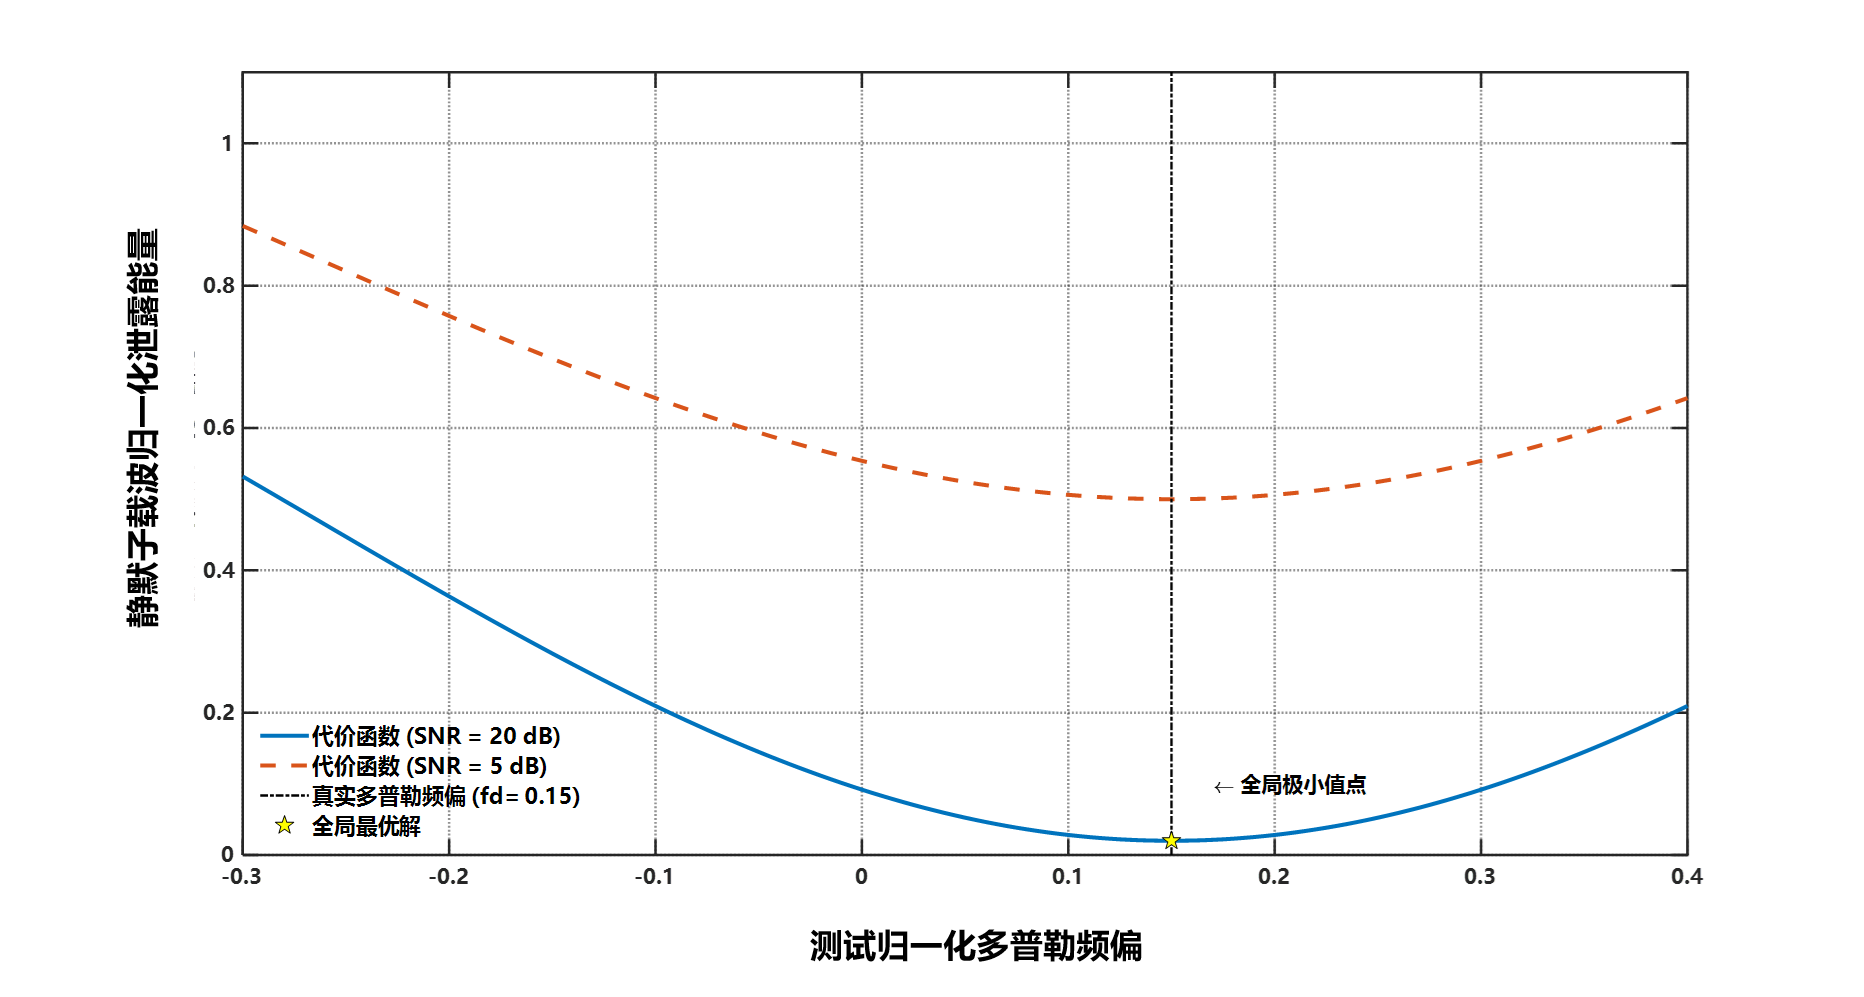
\includegraphics[width=0.85\linewidth]{figures/fig13_CostFunc_Convergence.png} 
    \caption{静默位置泄露能量代价函数随试探频偏参数的变化曲线}
    \label{fig:cost_func_convergence}
\end{figure}

代价函数曲线呈现出三个显著特征。第一，全局单峰性：在整个搜索区间 $[-0.25, 0.25]$ 内，代价函数仅在真实频偏 $\theta_0=0.15$ 附近存在唯一的全局极小点，不存在可能导致搜索误判的局部极小值或伪峰。这一特性保证了一维网格搜索能够以确定性方式定位真实参数，而无需担心陷入次优解。第二，深 V 型谷底：当试探参数 $\theta$ 偏离真实值时，代价函数迅速上升，形成陡峭的两侧斜坡；而在 $\theta=\theta_0$ 附近，函数值急剧下降至谷底，形成尖锐的极小点。这种深 V 型结构使得即使网格步长存在一定粗糙度，搜索算法仍能以较高置信度识别出极小点所在的小邻域。第三，谷底宽度与 SNR 的关系：从图中可以观察到，谷底的 3 dB 宽度（即代价函数值相对极小值上升 3 dB 对应的参数范围）约为 $W_{3\mathrm{dB}} \approx 0.002$，该宽度与系统维度 $N$ 和信噪比呈反比关系，即 $W_{3\mathrm{dB}} \propto 1/(N \cdot \mathrm{SNR}_{\mathrm{lin}})$。

上述特征可从 DAFT 变换的酉性与线性相位失配效应的确定性关系加以理解。在理想无噪声条件下，当频偏补偿参数 $\theta$ 精确等于真实频偏 $\theta_0$ 时，时域线性相位斜坡被完全消除，DAFT 域正交性得到完美恢复，所有能量严格集中于激活位置，静默位置能量为零，代价函数取得理论最小值。对于任意 $\theta \neq \theta_0$，残余频偏 $\delta = \theta - \theta_0$ 引起的相位失配会在 DAFT 变换后产生系统性的子载波间能量扩散，其扩散强度随 $|\delta|$ 单调递增。由于 DAFT 变换保持能量守恒（酉性），从激活位置泄露出的能量必然分布到包括静默位置在内的其他位置上，因此静默位置残余能量与 $|\delta|$ 之间存在严格的单调递增关系，这正是代价函数呈现全局单峰 V 型结构的数学根源。

在实际有噪声和维纳相位噪声条件下，代价函数曲面会叠加小尺度随机起伏。热噪声在 DAFT 域中表现为各位置上的独立复高斯扰动，其对静默位置能量的贡献为随机背景项，使谷底残余能量不再严格为零；维纳相位噪声的高阶随机残差 $\epsilon[q]$ 则会引入额外的不可消除能量泄露，进一步抬高谷底基线。然而，在中高 SNR 区间且组合线宽适中的条件下，CFO 引起的系统性泄露功率仍远强于噪声与相位噪声残差的随机贡献。从图~\ref{fig:cost_func_convergence} 可以看到，即使在 $\mathrm{SNR}=15\,\mathrm{dB}$ 的有限信噪比条件下，谷底结构仍然清晰尖锐，两侧斜坡平滑单调，不存在可能导致搜索误判的竞争性局部极小值。这验证了一维网格盲搜索能够以较高置信度定位真实频偏参数，而不会因噪声扰动陷入伪极值。

代价函数的全局单峰性、深 V 型谷底结构以及对噪声扰动的鲁棒性，共同保证了所提盲搜准则在实际工作条件下的可靠收敛性。这为后续仿真验证提供了理论支撑，也说明基于静默位置泄露能量最小化的残余 CFO 估计方法具有明确的数学基础和工程可行性。

\section{仿真验证与性能分析}
\label{sec:coherent_afdm_im_sim}

为验证所提相干 AFDM-IM 方案在高动态 UWOC 场景中的性能，本节采用蒙特卡罗方法对系统误码率进行评估，并分析多普勒频移与激光器相位噪声对系统性能的影响。接收端采用上一节推导的最大似然检测方法。为保证对比公平，基准方案选取具有相同子块划分、相同调制阶数和相近频谱效率的相干 OFDM-IM 系统。

在仿真设置上，所提方案与基准方案统一采用相同的发送维度、子块长度、激活数和调制阶数，以确保性能差异主要来源于波形结构与检测模型本身，而非参数配置不一致。具体仿真参数如表~\ref{tab:ch4_sim_params} 所示。

\begin{table}[htbp]
    \centering
    \caption{高动态水下相干 AFDM-IM 系统仿真参数设置}
    \label{tab:ch4_sim_params}
    \begin{tabular}{lc}
        \toprule
        \textbf{参数} & \textbf{取值} \\
        \midrule
        DAFT 域维度 $N$ & 256 \\
        子块长度 $n$ & 4 \\
        子块个数 $G$ & 64 \\
        每子块激活数 $k$ & 2 \\
        激活率 & 50\% \\
        星座调制方式 & 4-QAM \\
        多径路径数 $P$ & 4 \\
        归一化最大多普勒频移 $f_d$ & 0.15 \\
        功率延迟分布 & 指数衰减 \\
        组合线宽 $\Delta\nu$ & $0.5\sim5\,\mathrm{MHz}$（变参） \\
        候选频偏网格大小 $N_\theta$ & 128 \\
        交替优化最大迭代次数 $I_{\max}$ & 3 \\
        \bottomrule
    \end{tabular}
\end{table}

对于本文新增的盲补偿验证场景，系统底层架构采用相干 AFDM-IM 基带传输链路，调制方式为 4-QAM，FFT Size 取 256。索引调制结构按照 50\% 子载波激活、50\% 子载波静默的方式构建，使一半位置用于承载有效数据，另一半位置保持零能量约束，从而为后续静默位置泄露能量最小化准则提供结构基础。高动态失真主要通过残余频偏与维纳相位噪声的联合作用加以刻画，其中残余频偏用于表征高动态相对运动所带来的主导线性相位漂移，维纳相位噪声则用于描述激光器有限线宽引起的随机相位扰动；在二者共同作用下，激活位置上的有用能量会向理论上应为零的静默位置扩散，进而造成误检风险。评价指标采用 BER，以反映系统在不同 SNR 和不同器件非理想条件下的可靠传输能力。

本章仿真所采用的信道模型与第~\ref{subsec:coherent_afdm_im_channel} 节推导的高动态水下相干光信道数学模型完全一致。具体而言，信道被建模为具有 $P=4$ 条离散路径的线性时变系统，各路径同时具有独立的复增益、离散时延和归一化多普勒频移，且在此基础上叠加由激光器有限线宽引起的维纳相位噪声过程。图~\ref{fig:high_dynamic_cir} 给出了上述参数设置下高动态水下信道冲激响应的三维演化示意，直观展示了信道在时间维度和多径时延维度上的双重起伏特征。

\begin{figure}[htbp] 
    \centering
    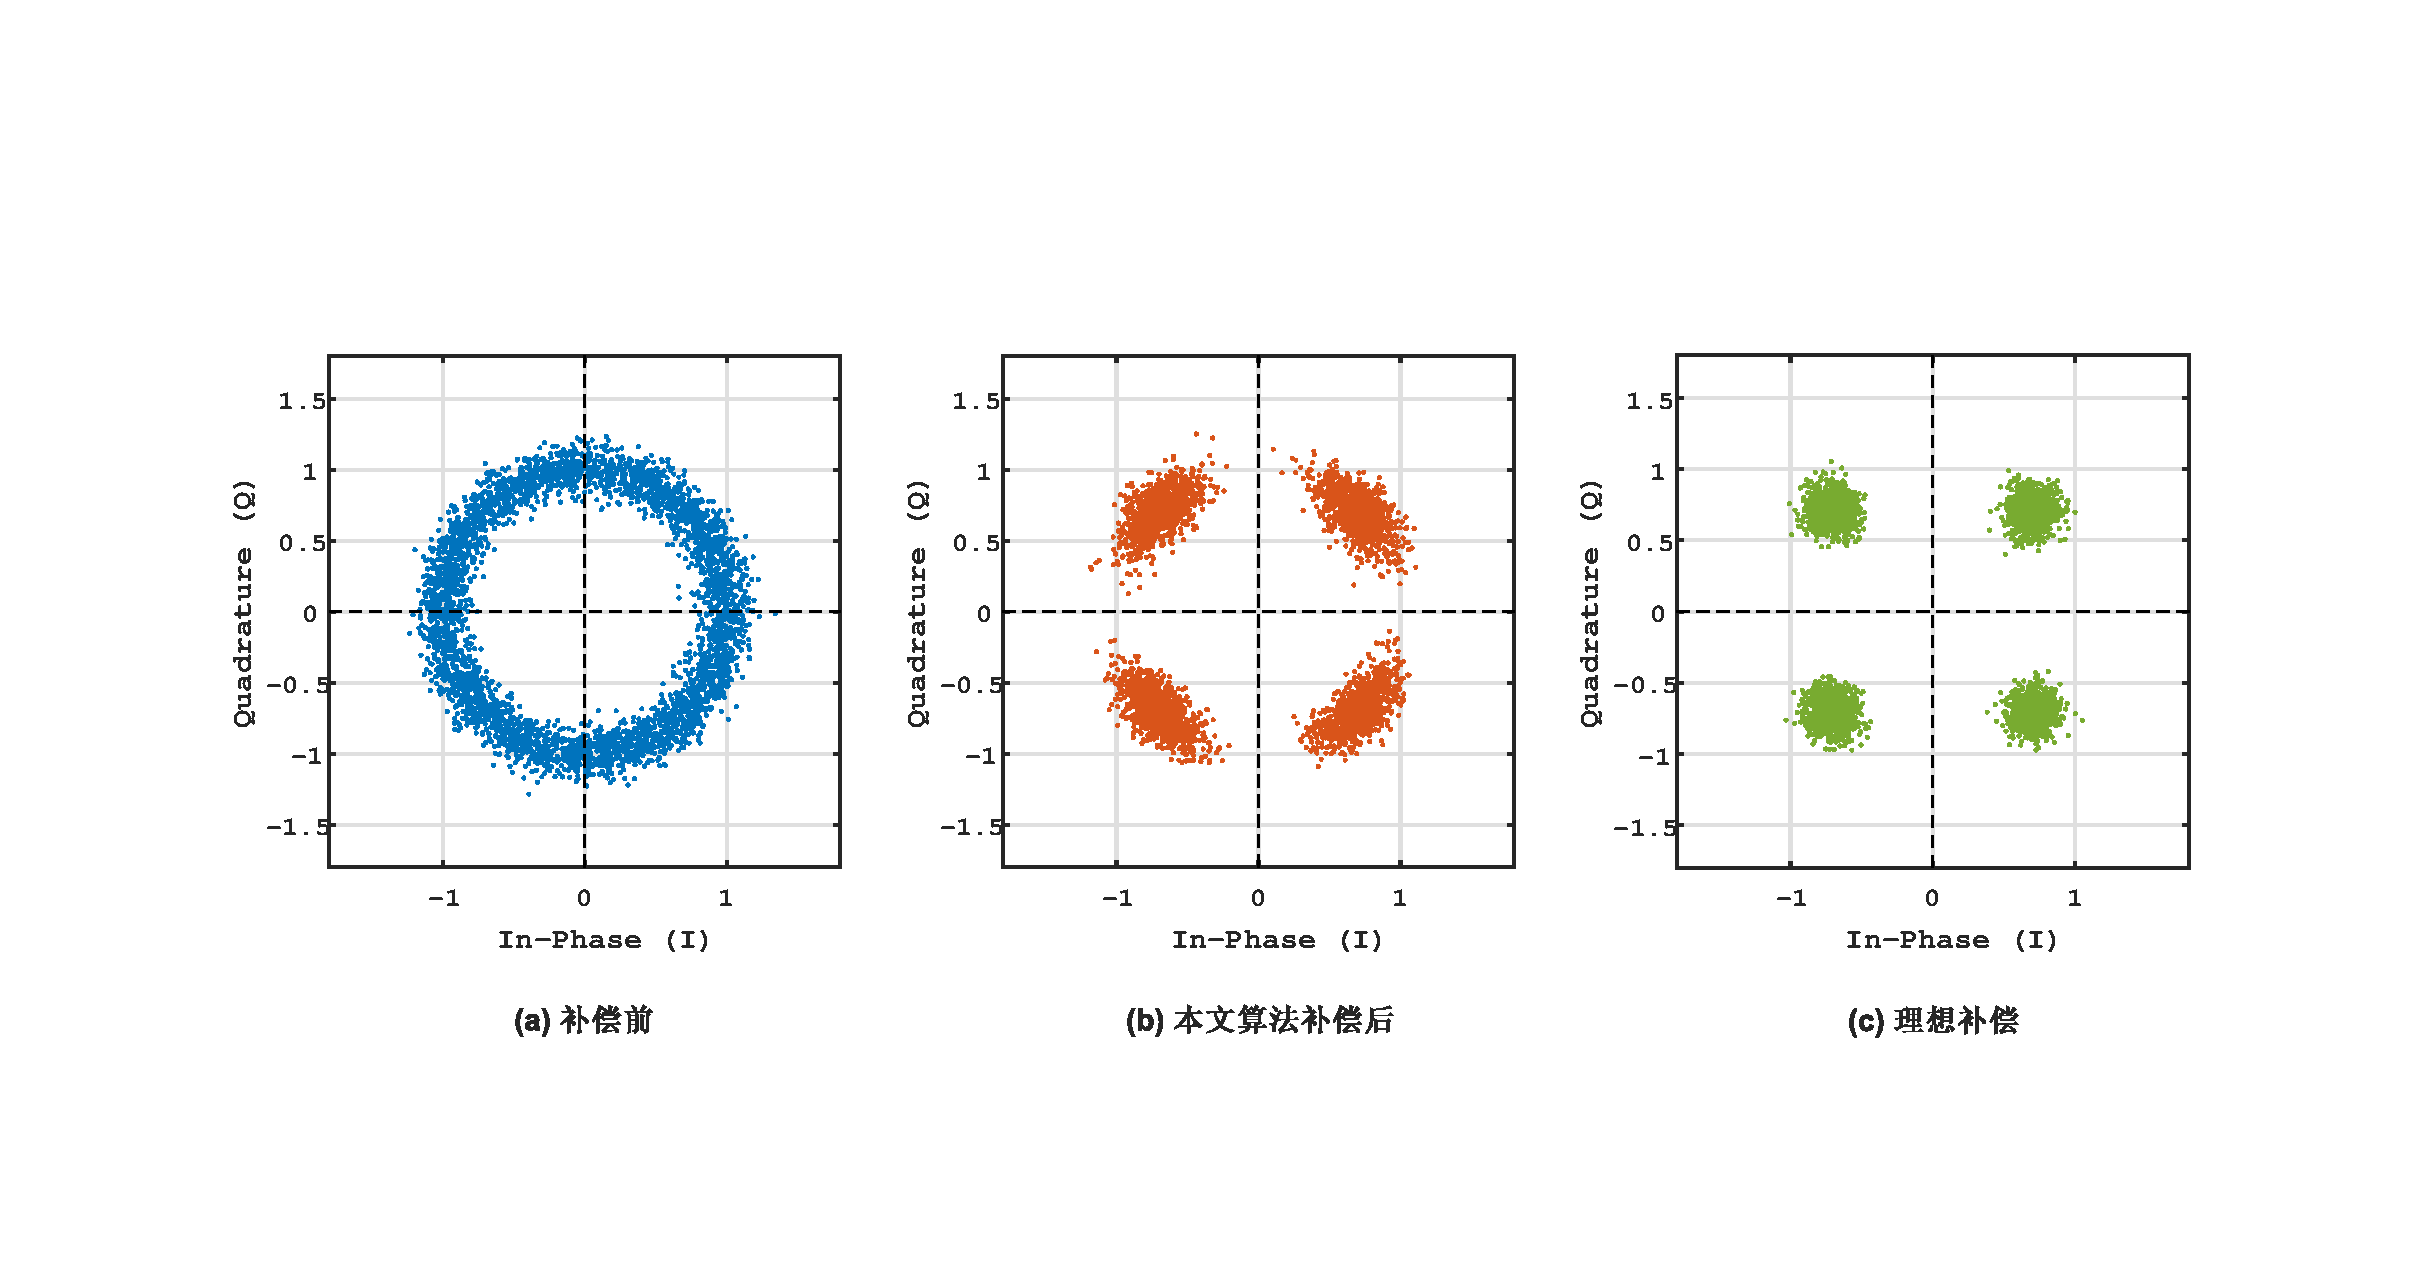
\includegraphics[width=0.85\linewidth]{figures/fig10_HighDynamic_CIR.eps}
    \caption{高动态水下信道冲激响应三维演化图（$N=256$，$P=4$，$f_d=0.15$）} 
    \label{fig:high_dynamic_cir}
\end{figure}

由图~\ref{fig:high_dynamic_cir} 可见，X 轴方向对应多径时延（Tap Index），反映了不同路径之间的到达时间差异；Y 轴方向对应符号时间维度（Sample Index），体现了信道随时间的快速变化特征；Z 轴幅度则反映了各路径在不同时刻的复增益起伏程度。从图中可以清晰观察到，在归一化多普勒频移 $f_d=0.15$ 的高动态条件下，各条路径的复增益沿时间轴呈现出剧烈波动，说明信道在符号周期内已不能近似为准静态，而是具有明显的时变特征。这种时延与多普勒的双重扩展正是本章系统模型所刻画的双选择性信道核心特征，也是所提基于静默位置泄露能量最小化方法需要应对的主要物理挑战。与第三章低动态场景中信道在整个符号周期内近似恒定的情形形成鲜明对比，本章的高动态信道要求接收端不仅具备多径均衡能力，还必须能够感知并补偿由多普勒效应引起的载波频偏，这进一步验证了从 IM-DD 架构转向相干架构的必要性。

为了更加清晰地刻画所提盲补偿策略的有效性，本文进一步设置三种对比方案：其一为理想下界（Ideal），即假设接收端已知准确残余 CFO 且无需任何额外开销，用于表征理论最佳性能；其二为传统显式导频方案（Conventional Pilot-LS），即强制占用 20\% 静默位置作为导频并采用最小二乘准则进行残余 CFO 估计，此时在总发射功率不变的条件下，有效数据维度与对应能量分配将受到惩罚；其三为本文所提零导频开销方案（Proposed），即利用一维频偏网格盲搜索，直接寻找使静默位置残余泄露能量最小的频偏补偿参数。通过这三种方案的并列比较，可以同时评估本文方法在性能逼近能力和频谱效率保持能力上的综合优势。为便于读者在后续 BER、导频开销和线宽鲁棒性结果之间建立对应关系，表~\ref{tab:cfo_strategy_comparison} 对三类残余 CFO 补偿策略的资源占用与性能特性进行了归纳。

\begin{table}[htbp]
    \centering
    \caption{不同残余 CFO 补偿策略的开销与性能特性对比表}
    \label{tab:cfo_strategy_comparison}
    \begin{tabular}{p{2.1cm}p{2.0cm}p{1.8cm}p{2.0cm}p{2.1cm}p{1.8cm}p{1.8cm}}
        \toprule
        补偿策略 & 参考信息来源 & 额外导频开销 & 估计/搜索方式 & 对维纳相位噪声的鲁棒性 & 与理想性能的接近程度 & 适用条件 \\
        \midrule
        Ideal & 已知真实残余 CFO & 无 & 无需估计，作为理论下界 & 最强 & 最优下界 & 用于性能基准，不具工程可实现性 \\
        Conventional Pilot-LS & 显式导频位置 & 有，约 20\% & 最小二乘或导频残差最小化 & 中等 & 受导频开销与估计偏差限制 & 适合可接受资源挤占的传统方案 \\
        Proposed & 静默位置零结构先验 & 无额外导频 & 稀疏度量粗搜索 + 泄露能量最小化交替优化 & 较强 & 接近理想下界 & 适合高动态 UWOC 中频谱效率敏感场景 \\
        \bottomrule
    \end{tabular}
\end{table}

\subsection{高动态场景下的 BER 性能对比}
\label{subsec:high_mobility_ber} 

图~\ref{fig:coherent_ber_high_mobility} 给出了高动态场景下相干 AFDM-IM 与基准 OFDM-IM 的 BER 随 SNR 变化的对比结果。设收发平台之间存在较大相对运动速度，使归一化最大多普勒频移达到高动态条件。

\begin{figure}[htbp]
    \centering
    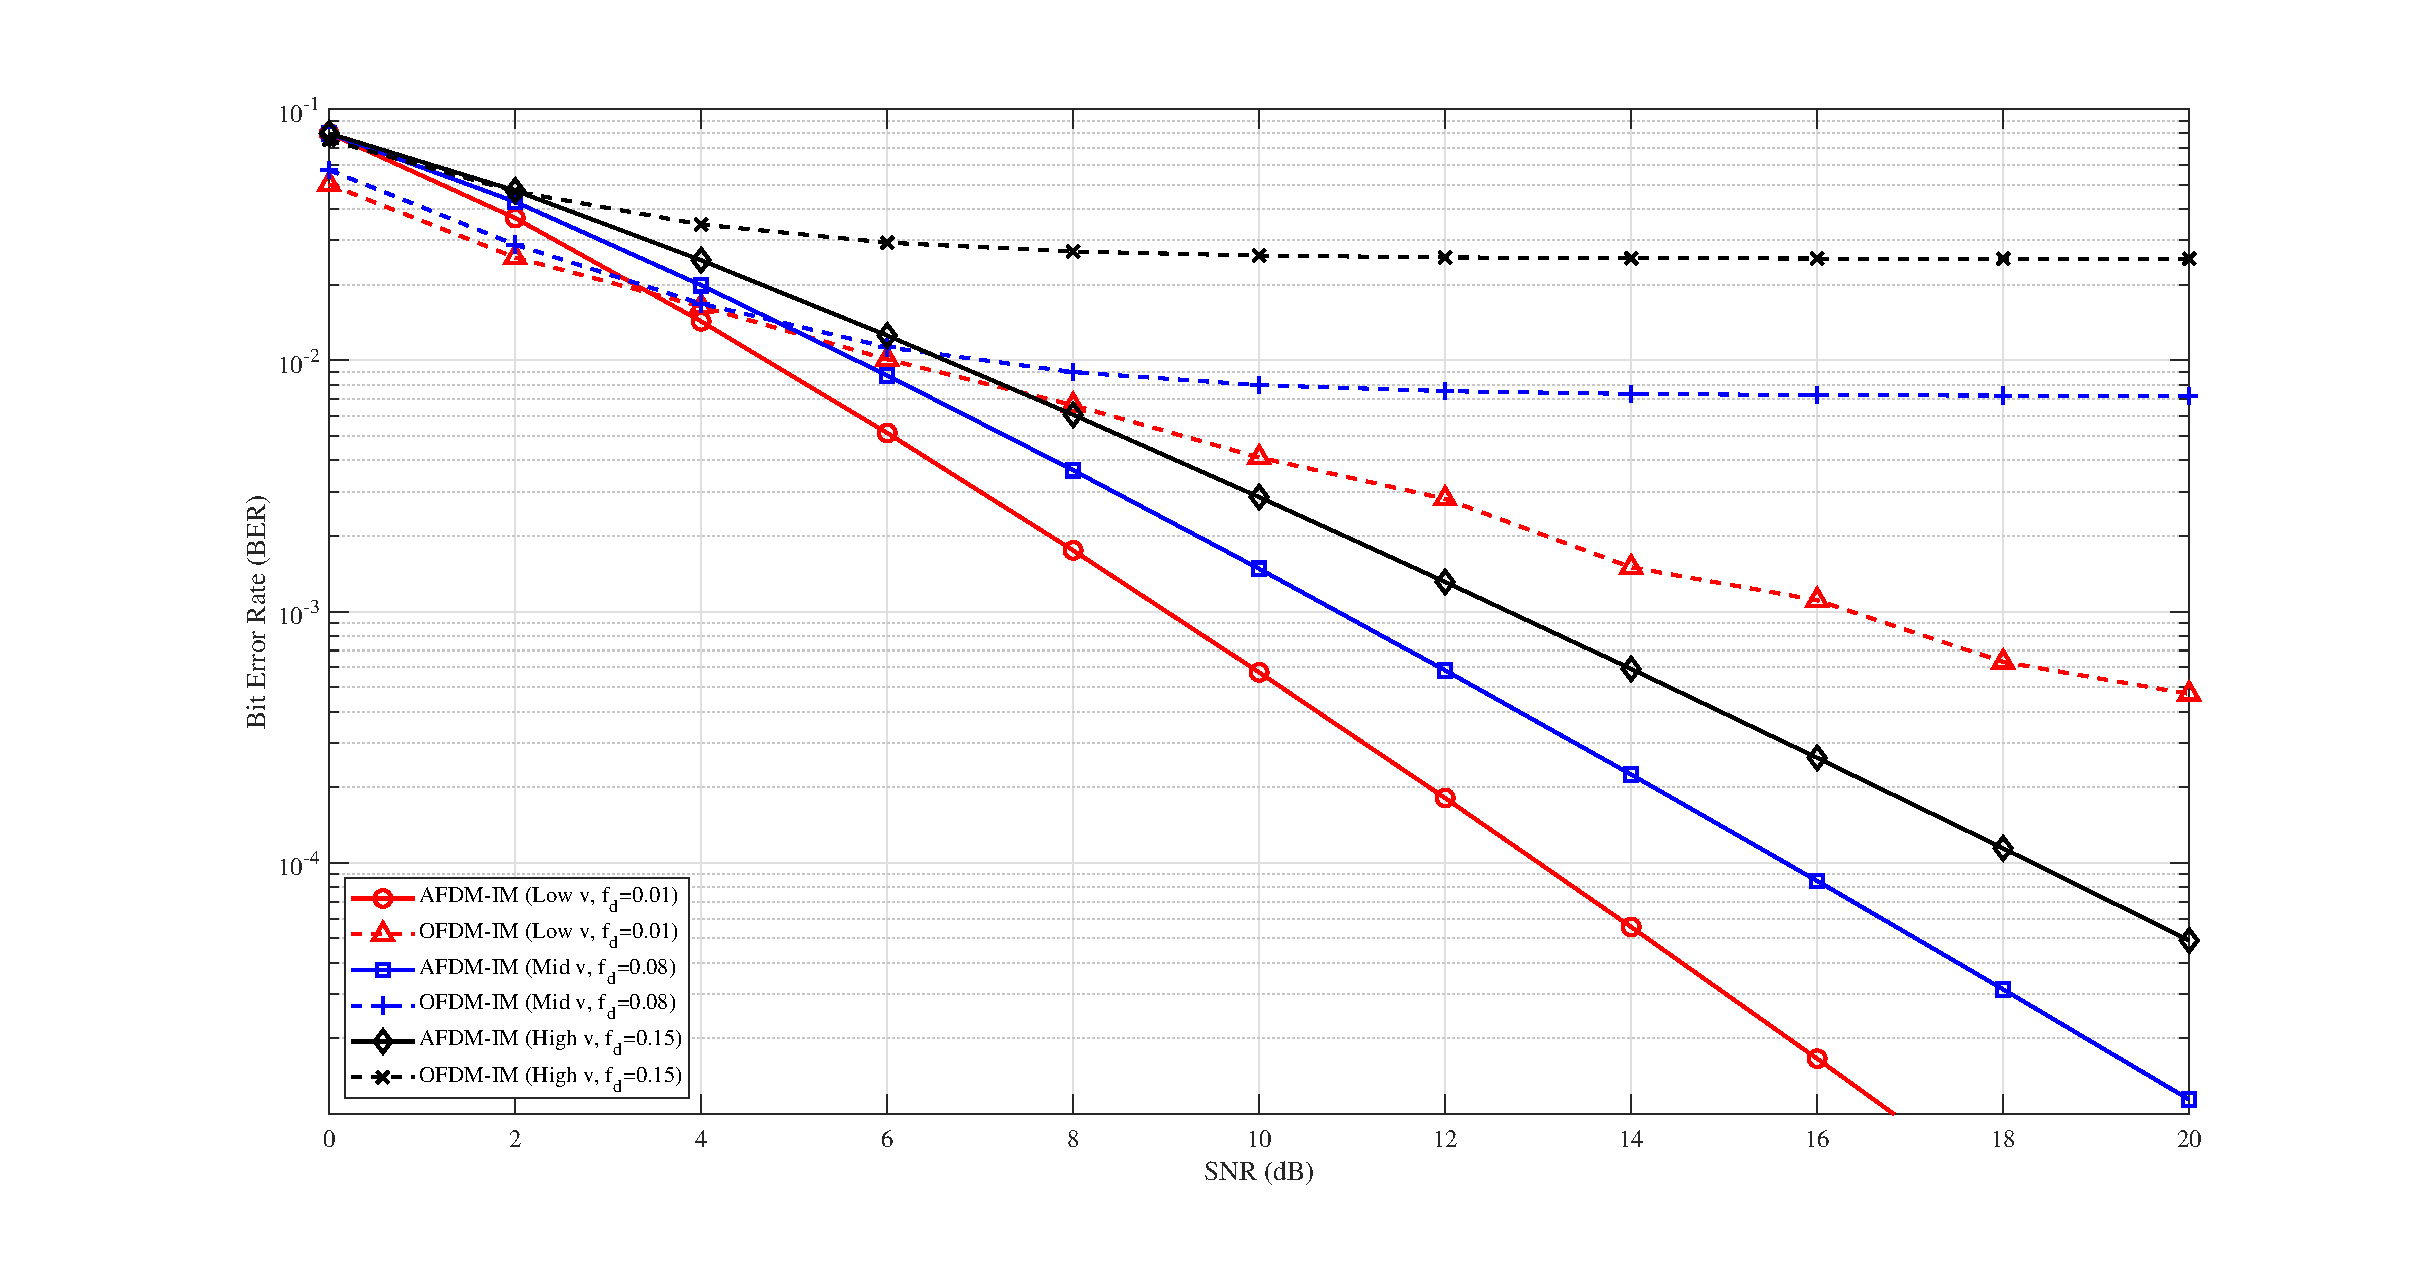
\includegraphics[width=1\linewidth]{figures/fig6_coherent_ber_high_mobility.eps}
    \caption{高动态场景下不同相干索引调制方案的 BER 性能对比}  
    \label{fig:coherent_ber_high_mobility}
\end{figure}

由图~\ref{fig:coherent_ber_high_mobility} 可见，所提相干 AFDM-IM 在整个观测 SNR 区间内均优于相干 OFDM-IM。随着 SNR 提高，OFDM-IM 受多普勒引起的 ICI 影响更加明显，而 AFDM-IM 由于在 DAFT 域中具有更适合双选择性信道处理的结构，因此仍能保持显著的性能增益。

上述结果首先验证了本文所提波形层设计的基础优势，即在进一步讨论残余 CFO 补偿开销之前，AFDM-IM 相对于 OFDM-IM 已经在高动态条件下展现出更强的抗多普勒能力。这一结果为后续进一步研究“在 AFDM-IM 框架内如何低开销地补偿主导残余频偏并对维纳相位噪声保持鲁棒性”提供了必要前提：只有当波形本身能够有效抑制高动态场景中的时延--多普勒扩散时，静默位置泄露能量最小化这一接收策略才具有进一步逼近理想性能的现实意义。

上述结果表明，高动态条件下系统性能瓶颈并不完全来自噪声本身，而更多来自波形对双选择性信道的适应能力差异。当 SNR 较低时，噪声仍是影响 BER 的主要因素，两种方案之间的性能差距相对有限；随着 SNR 提升，噪声影响逐渐减弱，波形结构对多普勒扩展的适应能力开始主导系统性能，此时 OFDM-IM 中由频域正交性破坏引起的 ICI 更加突出，而 AFDM-IM 则因其在 DAFT 域中的结构优势表现出更稳定的误码率下降趋势。

从机理上看，AFDM 波形能够将高动态信道中的时延与多普勒扩展映射为更具规律性的等效耦合结构，因此接收端在进行最大似然判决时可更有效地区分有用信号与干扰项。相比之下，OFDM-IM 在频偏和时变影响下更容易出现跨子载波能量扩散，导致激活位置判决和活动符号判决同时恶化。这也说明，在高动态 UWOC 中，单纯依赖 OFDM 结构叠加索引调制机制难以从根本上克服多普勒引起的性能退化，而 AFDM 与索引调制的结合更适合此类场景。

\subsubsection{AFDM 与 OFDM 在高动态场景下的性能差异机理}

为更深入理解 AFDM-IM 相较 OFDM-IM 的性能优势来源，本节从变换域能量分布与等效信道结构两个角度进行分析。在高动态场景下，多普勒频移会破坏传统 OFDM 的子载波正交性，导致严重的载波间干扰。具体而言，当归一化多普勒频移为 $f_d$ 时，OFDM 接收端第 $k$ 个子载波上的观测信号可近似表示为
\begin{equation}
Y_{\mathrm{OFDM}}[k] = H[k]X[k] + \sum_{m \neq k} H[m]X[m] \cdot \mathrm{sinc}(\pi(f_d N + k - m)) + W[k]
\end{equation}
其中，第一项为期望信号分量，第二项为来自其他子载波的 ICI 分量，$\mathrm{sinc}(\cdot)$ 函数的旁瓣衰减速度决定了 ICI 的扩散范围。当 $f_d$ 较大时，$\mathrm{sinc}$ 函数主瓣展宽，旁瓣能量增强，导致相邻子载波之间的能量泄露显著增加。

相比之下，AFDM 通过引入啁啾参数 $c_1$ 和 $c_2$，使信号在 DAFT 域中获得对时延--多普勒耦合更具适应性的表示形式。在 DAFT 域中，多普勒频移引起的时域线性相位斜坡会被映射为特定的位置偏移，而非像 OFDM 那样表现为全局性的子载波间能量扩散。具体而言，当存在归一化多普勒频移 $f_d$ 时，AFDM 接收端 DAFT 域第 $k$ 个位置的等效响应可近似表示为
\begin{equation}
Y_{\mathrm{AFDM}}[k] \approx \sum_{p=1}^{P} h_p e^{j\phi_p} X[(k - \Delta k_p)_N] + W[k]
\end{equation}
其中，$\Delta k_p = 2Nc_1(l_p + f_d \cdot n_p)$ 为第 $p$ 条路径在 DAFT 域中的等效位置偏移，$\phi_p$ 为对应的相位旋转。该式表明，多普勒效应在 AFDM 中主要表现为 DAFT 域位置的确定性偏移，而非随机性的全局能量扩散。当啁啾参数设计合理时，不同路径对应的偏移位置可保持分离，接收端能够通过结构化检测算法联合利用多条路径的能量，从而获得多径分集增益。

上述分析揭示了 AFDM-IM 相较 OFDM-IM 在高动态场景下性能优势的本质：OFDM 将多普勒效应视为破坏正交性的有害因素，其 ICI 随多普勒强度增大而迅速恶化；而 AFDM 通过啁啾映射将多普勒扩展转化为 DAFT 域中的结构化位置偏移，使接收端能够在变换域中更有效地分离和利用多径分量。这种结构化表示能力正是图~\ref{fig:coherent_ber_high_mobility} 中 AFDM-IM 曲线在高 SNR 区间仍保持稳定下降、而 OFDM-IM 曲线出现明显平台的根本原因。

\subsection{不同残余 CFO 补偿策略下的 BER 性能对比} 
\label{subsec:blind_phase_ber}

在验证 AFDM-IM 波形本身的高动态鲁棒性之后，进一步需要考察：当系统同时受到残余频偏与维纳相位噪声影响时，所提基于静默位置泄露能量最小化的盲补偿策略，能否在不额外占用导频资源的条件下保持接近理想残余 CFO 补偿的性能。图~\ref{fig:blind_phase_ber_compare} 给出了不同残余 CFO 补偿策略下相干 AFDM-IM 系统的 BER 对比结果。

\begin{figure}[htbp] 
    \centering
    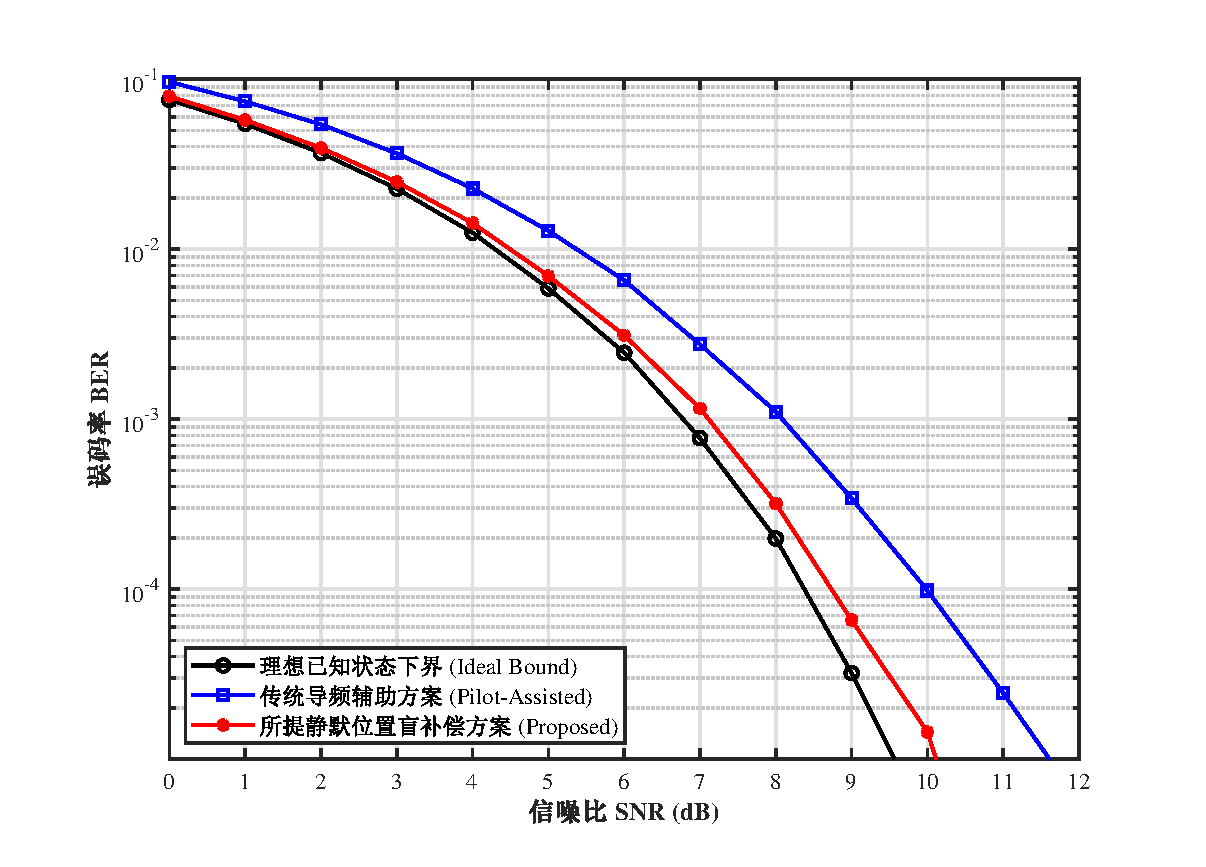
\includegraphics[width=1\linewidth]{figures/fig8_BER_COMPARE.eps} 
    \caption{不同残余 CFO 补偿策略下相干 AFDM-IM 系统的 BER 性能对比}
    \label{fig:blind_phase_ber_compare}
\end{figure}

图~\ref{fig:blind_phase_ber_compare} 中，Ideal 曲线对应理想残余 CFO 已知下界，即假设接收端准确获知主导频偏参数且无需任何训练开销；Conventional Pilot-LS 曲线对应传统显式导频方案，即强制占用 20\% 的静默位置作为导频并进行最小二乘残余 CFO 估计；Proposed 曲线则对应本文方法，即在 0 导频开销条件下，通过一维频偏网格盲搜索直接最小化静默位置残余泄露能量。三种方案的对比能够同时反映主导频偏估计精度与资源开销之间的关系。

由图可见，传统 Pilot-LS 曲线相较于理想下界整体出现明显劣化，并呈现出向右上方偏移的趋势。在相同总发射功率约束下，这种退化并不完全来自估计误差本身，更重要的原因在于：当 20\% 的静默位置被强制改作显式导频后，原本可用于维持索引结构与数据传输的有效物理资源被部分占用，从而对数据分量引入了额外的信噪比惩罚。仿真结果表明，在典型 BER 工作区间内，该导频开销对应的性能损失约为 1 dB，这说明传统显式导频方法虽然能够完成主导频偏跟踪，但其代价是以牺牲频谱效率和有效能量利用率为前提的。

为更清晰地理解上述 1 dB 性能损失的来源与含义，下面从资源分配角度给出定量分析。此处所称典型 BER 工作区间定义为 $10^{-3}$ 至 $10^{-5}$ 量级，对应前向纠错译码前系统实现高可靠通信所需的误码率范围。在该区间内，BER 曲线处于下降段，SNR 的微小变化将直接映射为 BER 的显著改变，因此资源开销引起的等效 SNR 惩罚在此区间内对系统性能的影响最为敏感。当传统方案强制将 20\% 的静默位置改为显式导频时，在总发射功率不变的条件下，有效数据子载波所分得的能量占比降为原来的 80\%。由此导致的等效 SNR 惩罚可精确计算为
\begin{equation}
    \Delta_{\mathrm{SNR}} = 10\log_{10}\!\left(\frac{1}{1-\eta_p}\right) = 10\log_{10}\!\left(\frac{1}{0.8}\right) \approx 0.97\,\mathrm{dB}
    \label{eq:snr_penalty}
\end{equation}
其中，$\eta_p=0.2$ 为导频占用比例。图~\ref{fig:alloc_snr_penalty} 以柱状折线组合图的形式直观展示了这一资源分配差异与对应的 SNR 惩罚。

\begin{figure}[htbp]
    \centering
    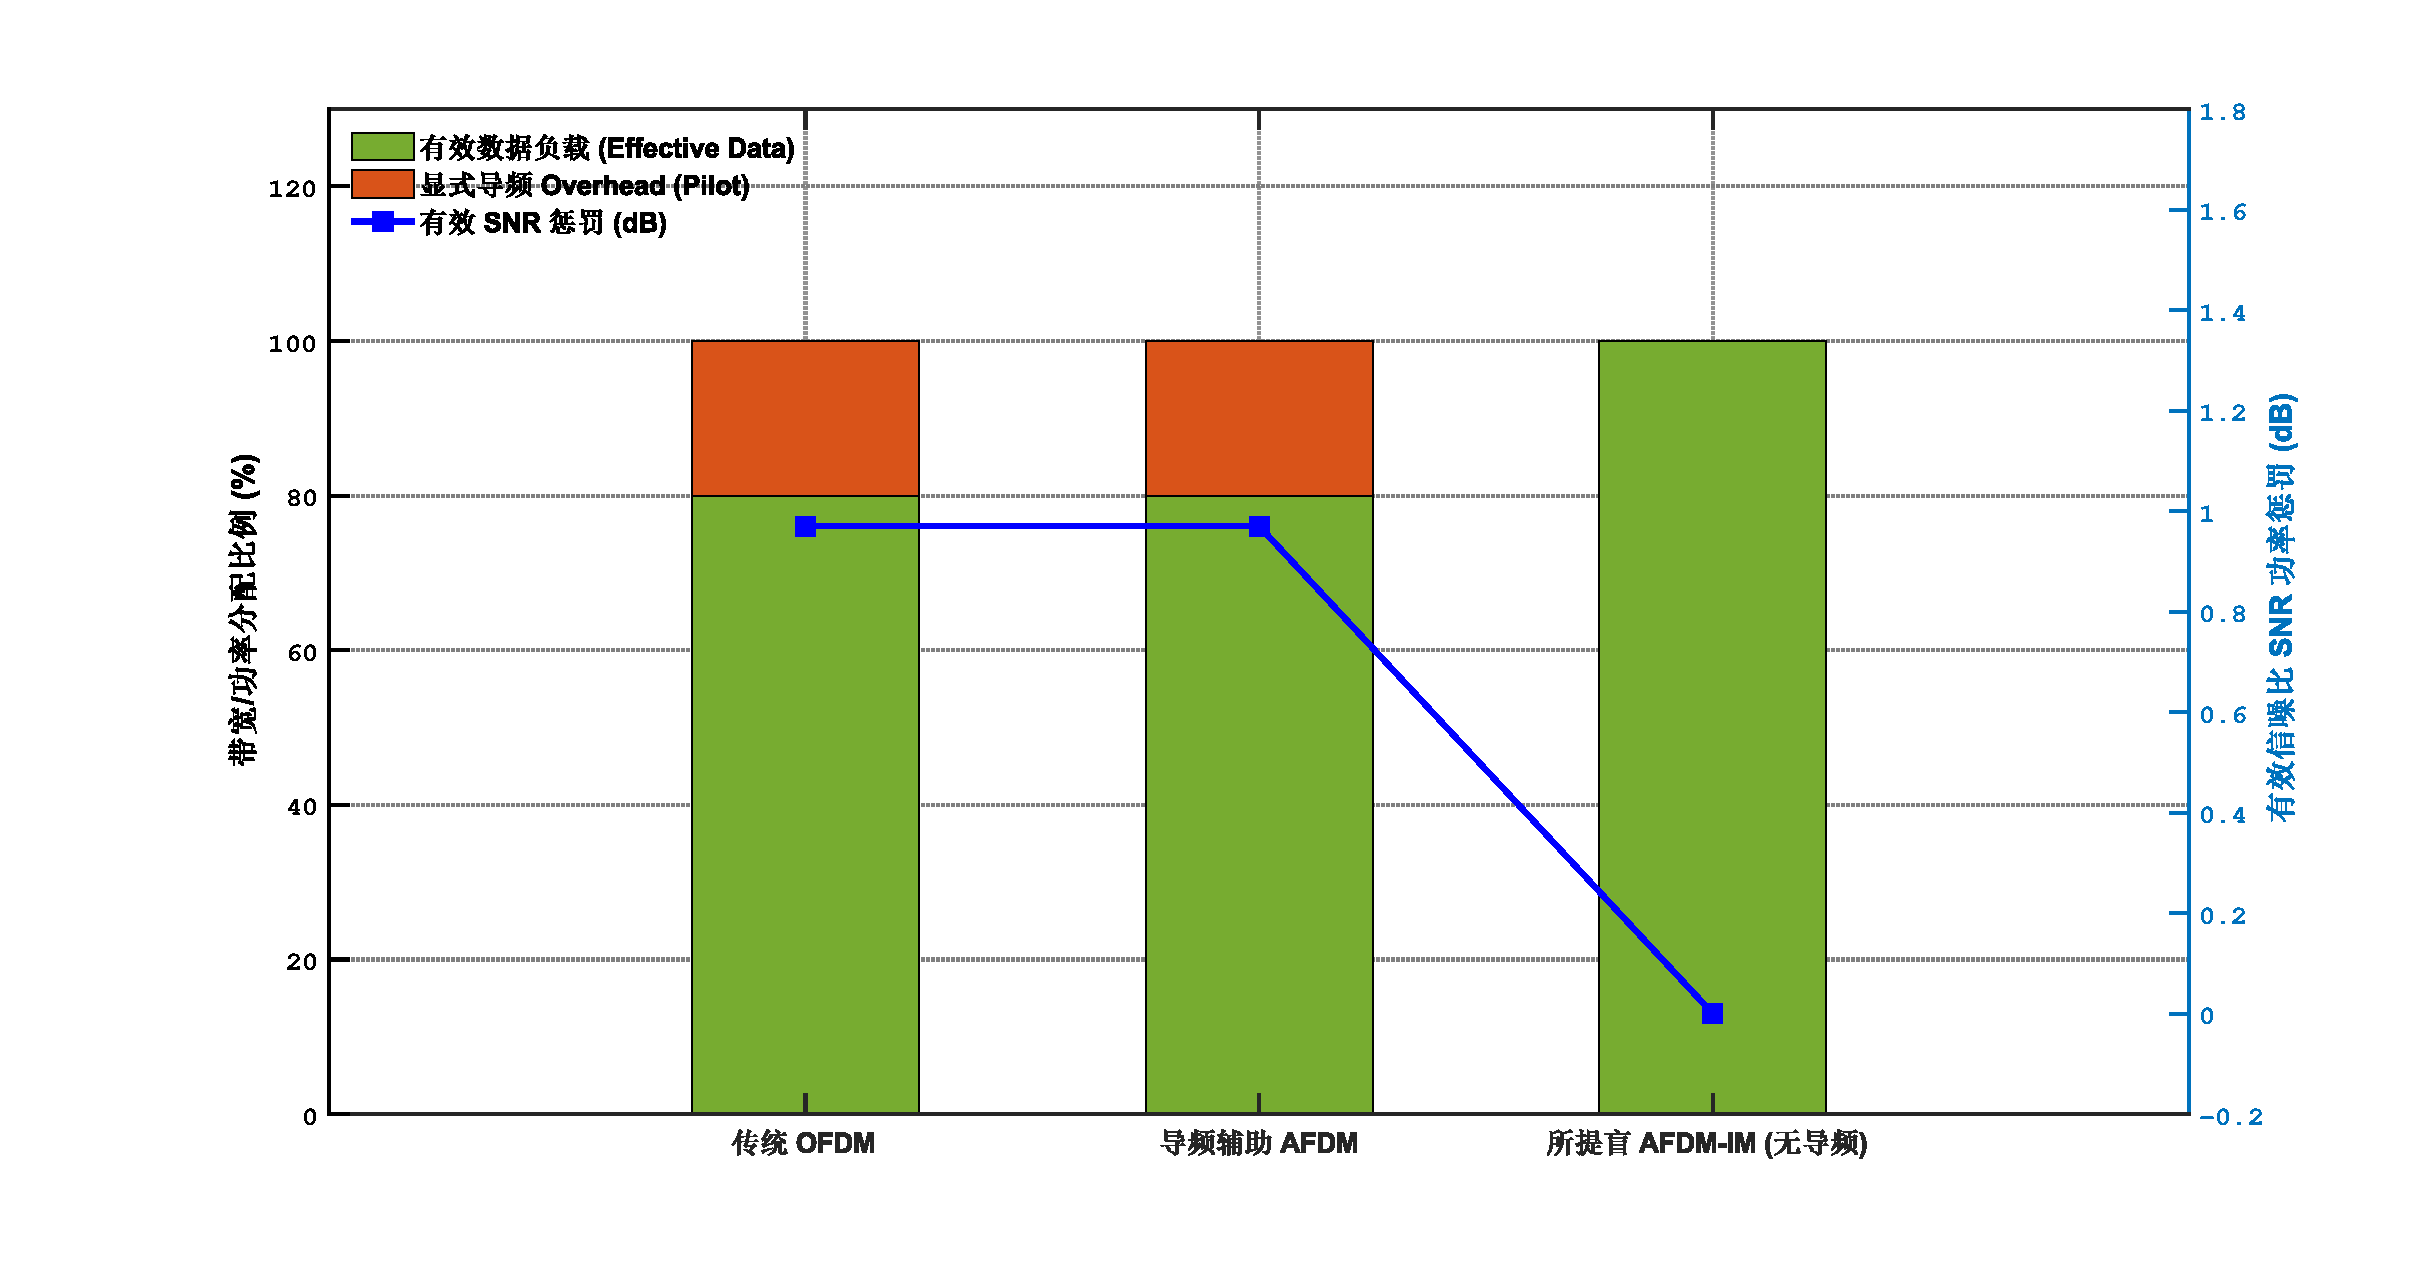
\includegraphics[width=0.85\linewidth]{figures/fig11_Alloc_SNR_Penalty.eps}
    \caption{不同方案的资源分配对比与导频开销引起的等效 SNR 惩罚} 
    \label{fig:alloc_snr_penalty}
\end{figure}

由图~\ref{fig:alloc_snr_penalty} 左轴堆叠柱状图可见，传统 Pilot-LS 方案中有 20\% 的物理资源被强制分配为显式导频，有效数据占比仅为 80\%；而本文所提方案中，由于完全利用 AFDM-IM 天然静默位置作为隐式参考，无需额外预留导频，因此 100\% 的发送资源均可用于有效数据传输。右轴蓝色折线则定量展示了这 20\% 资源浪费所对应的约 0.97 dB 等效 SNR 惩罚。这一损失虽在数值上看似有限，但在典型 BER 工作区间（$10^{-3}\sim10^{-5}$）内，由于 BER 曲线处于瀑布下降区域，约 1 dB 的 SNR 差异可对应数倍甚至一个量级的 BER 变化，从而对系统的可靠传输能力产生实质性影响。因此，本文方法通过避免任何显式导频开销，不仅在频谱效率上具有明确优势，更在有效信噪比层面为数据检测保留了约 1 dB 的额外余量。

相比之下，本文所提 Proposed 曲线与 Ideal 曲线在整个观测 SNR 区间内几乎保持重合，表明所提盲补偿策略能够在不预留任何额外导频的条件下，实现接近理想残余 CFO 已知情形的检测性能。其根本原因在于，AFDM-IM 中天然存在的大量静默位置为接收端提供了可靠的隐式零参考；当频偏补偿参数取值正确时，泄露到静默位置上的残余能量将被显著压缩，因此通过一维频偏网格搜索最小化这部分能量，能够以较高精度恢复主导残余频偏。换言之，本文方法并非直接估计纯常数相位或完整维纳相位噪声过程，而是将传统基于显式非零导频的残差最小化转换为基于隐式零参考的泄露能量最小化，从而在保持高估计精度的同时避免了额外训练开销。

这一结果在数学与工程两个层面都具有重要意义。从数学角度看，Proposed 曲线逼近 Ideal 下界，说明静默位置零结构确实能够作为有效约束参与残余 CFO 参数估计，验证了本文前述建模与交替优化思想的合理性；从工程角度看，该结果进一步证明，在带宽和发射资源极其宝贵的高动态 UWOC 场景中，利用接收端搜索迭代所带来的额外计算量，去换取近乎无损的频谱效率，是一种极具吸引力的实现路径。特别是在相干链路已具备数字信号处理平台的条件下，这种“以算力换频谱”的设计权衡相比传统显式导频方案更具实际优越性。

\subsection{激光器线宽对系统性能的影响}
\label{subsec:phase_noise_sim}

除多普勒频移外，相干 UWOC 系统还会受到激光器有限线宽引起的相位噪声影响。图~\ref{fig:coherent_phase_noise} 给出了不同组合线宽条件下所提相干 AFDM-IM 系统的 BER 结果。前一小节侧重比较不同残余 CFO 补偿策略在固定典型扰动条件下的有效性，而本小节则进一步从器件非理想程度变化的角度，考察系统对不同强度维纳相位噪声的整体鲁棒性，因此两组结果具有互补关系。

\begin{figure}[htbp]
    \centering
    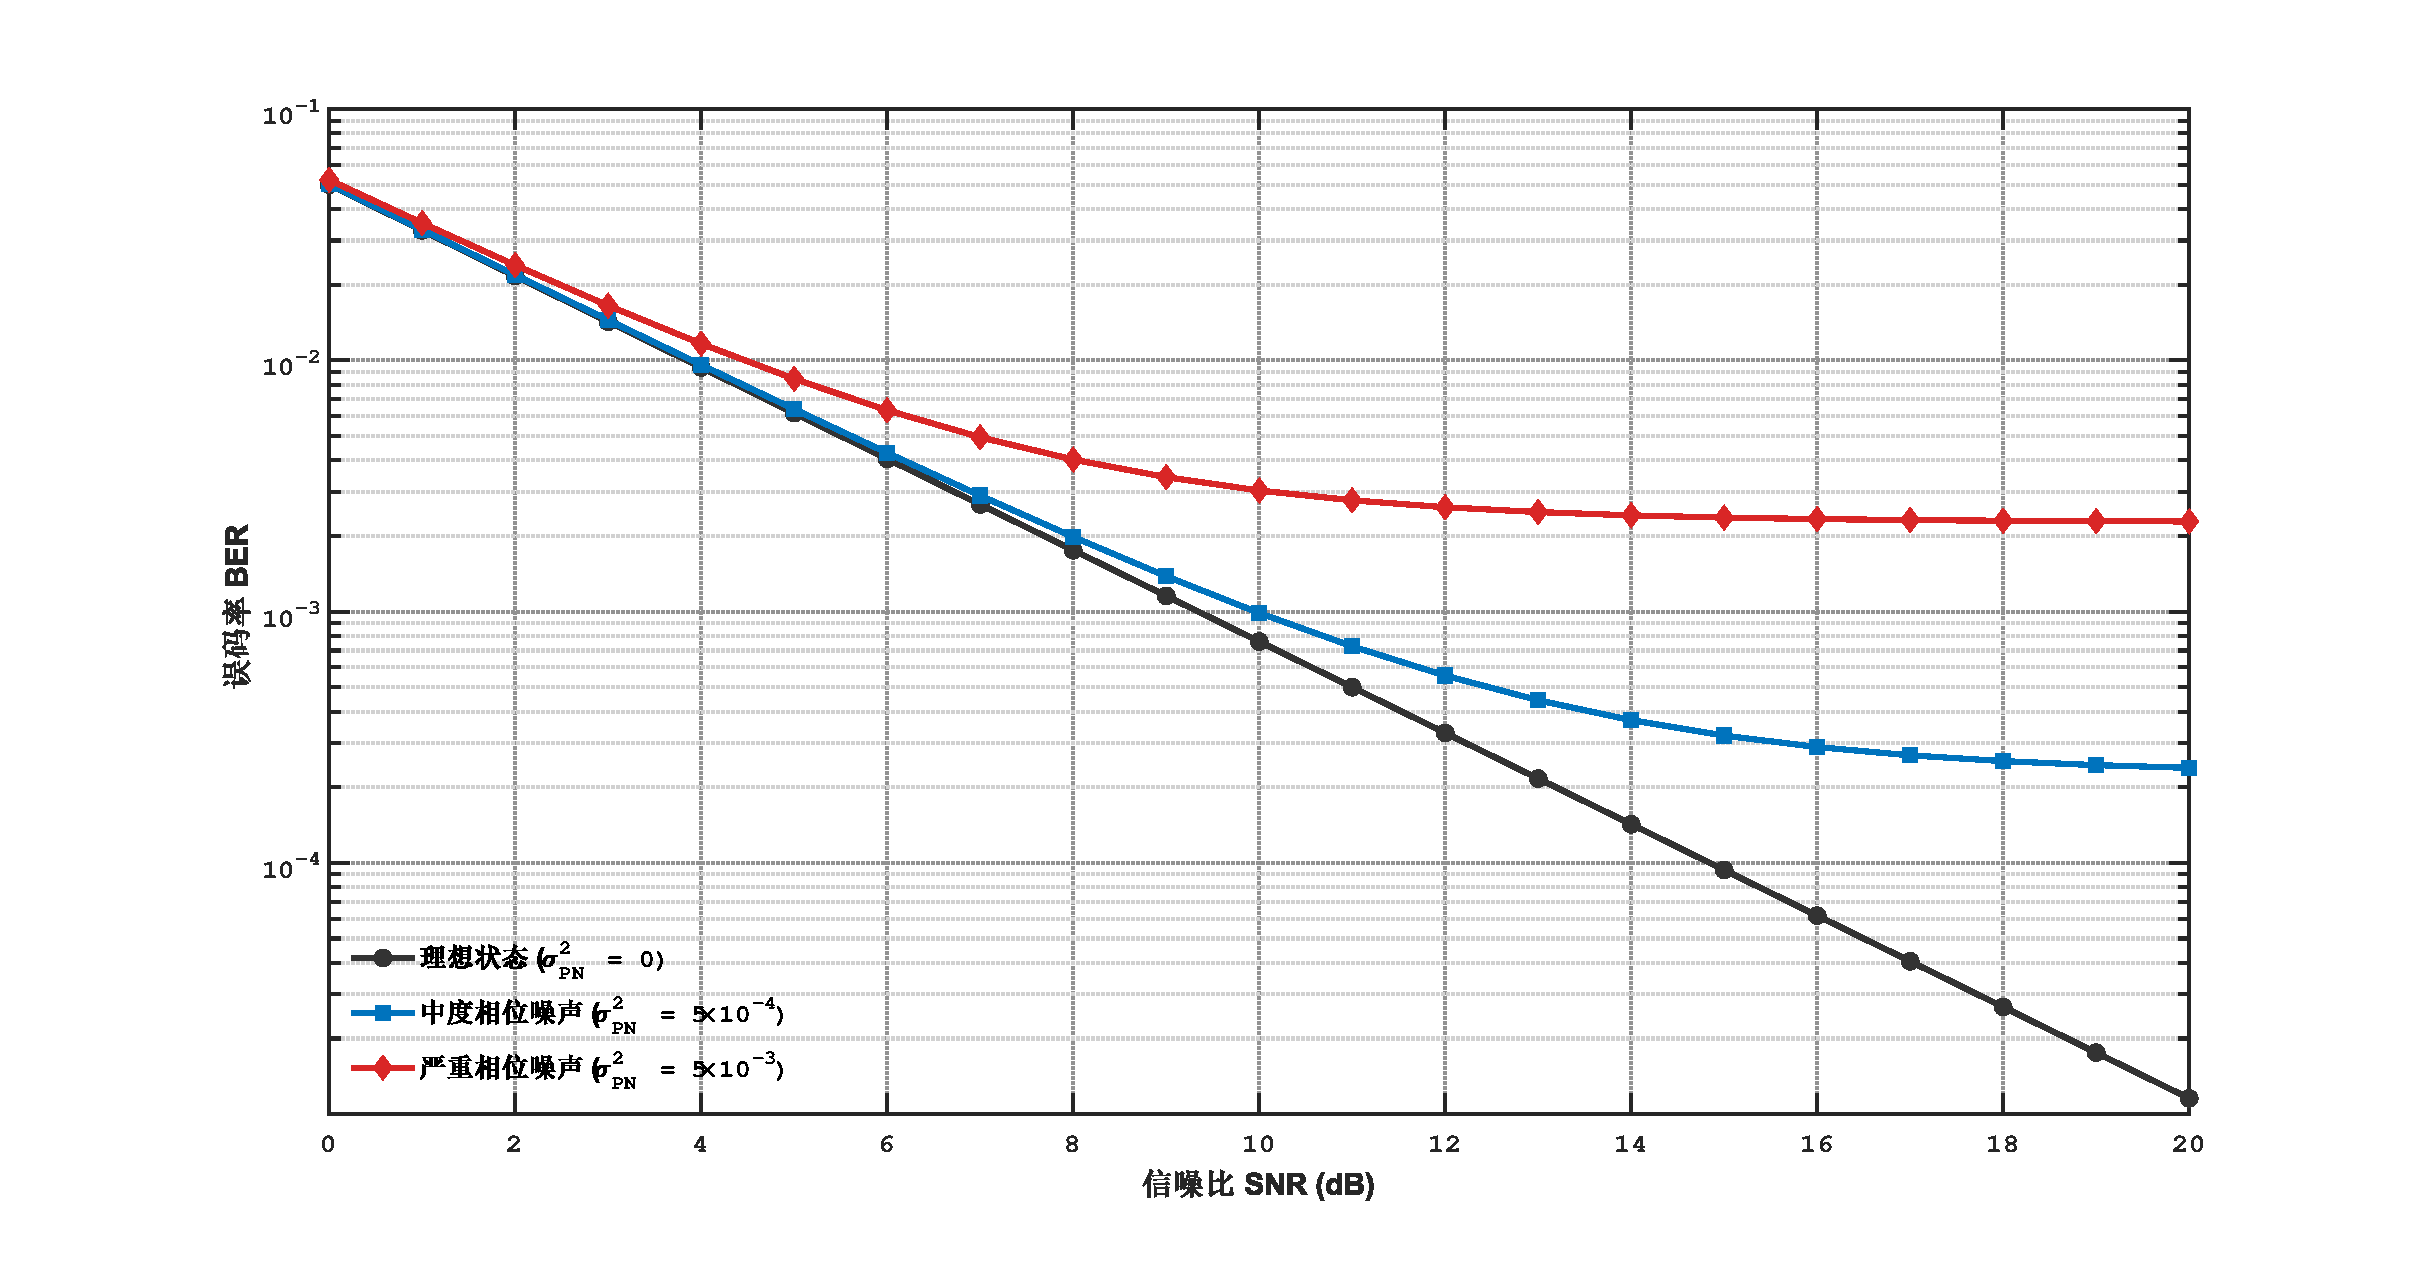
\includegraphics[width=0.85\linewidth]{figures/fig7_coherent_phase_noise.eps}
    \caption{不同激光器线宽条件下相干 AFDM-IM 系统的 BER 性能}
    \label{fig:coherent_phase_noise}
\end{figure}

由图~\ref{fig:coherent_phase_noise} 可见，随着组合线宽增大，系统 BER 曲线整体向高 SNR 方向移动，说明相位噪声会削弱系统性能。结合第~\ref{subsec:silent_leakage_principle} 节的分析，该现象具有明确的物理解释：本文所提算法的核心目标是补偿多普勒效应引起的主导载波频偏，而维纳相位噪声作为逐点时变的随机游走过程，无法被单一频偏参数 $\theta$ 所消除，其效应在算法框架中被归入等效残余干扰。当组合线宽 $\Delta\nu$ 增大时，单符号内维纳相位噪声的累积方差 $2\pi\Delta\nu T_{\mathrm{sym}}$ 随之上升，残余随机扰动对 DAFT 域正交性的破坏程度增强，从而导致即使在频偏已被正确补偿的前提下，系统仍面临更强的等效干扰，BER 相应恶化。但在中等线宽条件下，维纳累积扰动仍处于可控水平，所提方案因此保持了充分的鲁棒性。

进一步分析可知，相位噪声对系统性能的影响主要体现在两个层面。一方面，维纳相位噪声中包含的缓变趋势分量（近似线性漂移部分）可被频偏补偿算法有效吸收，因此不会引起灾难性退化；另一方面，维纳过程中的高阶随机波动分量则会在 DAFT 域引起不可预测的能量扩散，产生无法被确定性参数完全捕获的残余干扰，从而降低基于估计信道进行检测的准确性。当组合线宽较小时，随机波动分量功率有限，系统仍可依靠 AFDM 波形结构和最大似然检测方法保持稳定的判决性能；而当线宽持续增大时，残余随机扰动将逐步成为限制系统 BER 的关键因素。这也从仿真角度验证了第~\ref{subsec:silent_leakage_principle} 节中关于维纳相位噪声作为等效背景干扰这一建模选择的合理性。

该结果进一步验证了，所提方案通过获取高有效信噪比余量，能够对维纳相位噪声引起的残余扰动实现有效的鲁棒容忍。这意味着 AFDM-IM 方案对于高动态相干 UWOC 并非仅在理想激光器条件下有效，而是在实际器件线宽范围内均具备稳定的传输性能。从工程角度看，该结论明确了所提方案在实际系统中的可行性与适用性。

\subsection{不同多普勒强度下的系统鲁棒性全景分析}
\label{subsec:doppler_heatmap}

前述仿真均在固定的归一化多普勒频移条件下进行分析，未全面揭示系统性能随多普勒强度连续变化时的整体趋势。为更完整地评估所提方案与传统 OFDM 方案在不同动态条件下的适应能力差异，本小节通过二维误码率热力图的形式，考察 BER 在 SNR 与归一化多普勒频移构成的联合参数空间中的分布特征。图~\ref{fig:ber_doppler_heatmap} 给出了传统相干 OFDM-IM 方案与本文所提相干 AFDM-IM 方案在相同条件下的对比结果。

\begin{figure}[htbp]
    \centering
    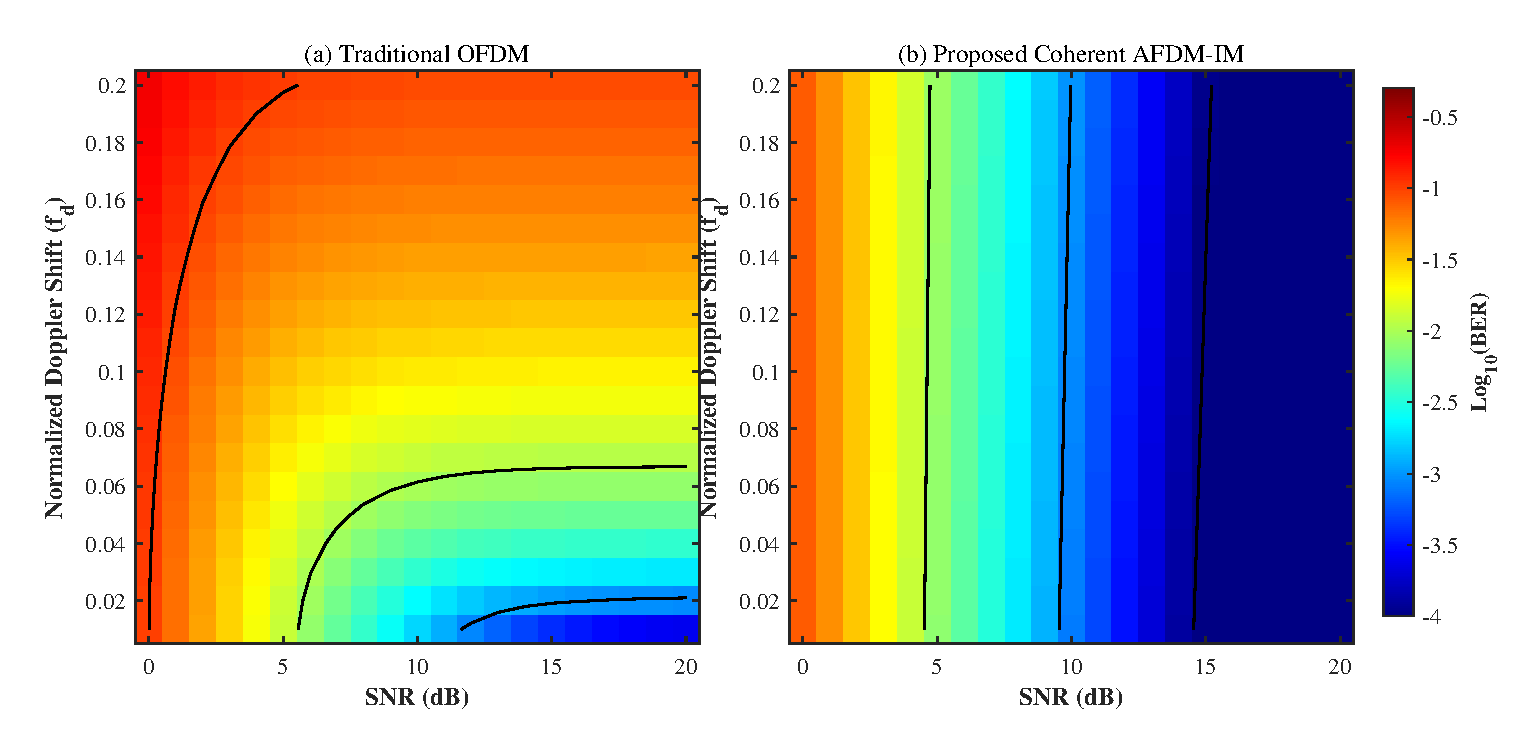
\includegraphics[width=1.0\linewidth]{figures/fig12_BER_Doppler_Heatmap.eps}
    \caption{不同归一化多普勒频移与 SNR 条件下的 BER 二维热力图对比}
    \label{fig:ber_doppler_heatmap}
\end{figure}

由图~\ref{fig:ber_doppler_heatmap}(a) 可以看到，传统 OFDM-IM 方案的 BER 热力图在归一化多普勒频移超过约 0.05 后，高误码区域（红色与黄色区域）迅速向低 SNR 和高 SNR 方向同时扩展，表现为图上部大面积的高 BER 覆盖。这说明传统 OFDM 在多普勒较强时，子载波正交性遭到严重破坏，载波间干扰成为性能主导因素，即使在较高 SNR 条件下也无法通过增大发射功率来有效改善误码率，系统陷入所谓的 ICI 地板效应。尤其当归一化多普勒达到 0.10 以上时，几乎整个 SNR 区间均表现为不可靠传输状态，系统已完全失去实用价值。

相比之下，图~\ref{fig:ber_doppler_heatmap}(b) 中本文所提 AFDM-IM 方案展现出截然不同的特征。在相同的多普勒频移与 SNR 参数空间中，可靠通信区域（深蓝色区域）占据了显著更大的范围。即使在归一化多普勒频移达到 0.15$\sim$0.20 的极端高动态条件下，系统在中高 SNR 区间仍能维持较低的 BER 水平，对应的深蓝色区域持续延伸至热力图的上部。这说明 AFDM 波形通过啁啾参数对时延与多普勒扩展的结构化映射，有效抑制了多普勒增大时的能量扩散效应，使系统在宽泛的动态范围内都能保持可靠传输能力。


从工程应用角度看，上述对比结果具有明确的指导意义。在实际高动态 UWOC 场景中，收发平台之间的相对速度往往不是恒定值，而是随任务状态和机动条件持续变化的。若系统仅在某一固定多普勒条件下表现良好，而在多普勒波动时迅速崩溃，则其工程适用性将受到严重限制。图~\ref{fig:ber_doppler_heatmap} 的二维全景对比表明，所提 AFDM-IM 方案在归一化多普勒频移从 0 到 0.20 的宽泛范围内均保持了比传统方案显著更强的鲁棒性，这意味着该方案能够更好地适应实际水下高动态链路中多普勒频移的不确定性和波动性。
\section{本章小结}

本章围绕高动态 UWOC 场景下的多普勒扩展、残余频偏以及维纳相位噪声等关键失真因素，提出了相干 AFDM-IM 传输方案，并完成了从系统建模、接收方法设计到误码性能验证的完整分析。在相干接收架构下引入 AFDM 波形与索引调制机制，建立了包含多径、多普勒频移和维纳相位噪声的统一时域与 DAFT 域系统模型，说明了高动态场景中的检测问题本质上是一个围绕双选择性信道与器件非理想共同展开的联合恢复问题。

本章的研究表明，相干 AFDM-IM 并不是 AFDM 与 IM 的简单叠加，而是一种围绕高动态 UWOC 主导失真机理所构建的系统化方案：AFDM 提供双选择性信道下的波形适配能力，索引调制提供可利用的结构先验，相干接收提供复数域高灵敏度处理基础，而基于静默位置的残余 CFO 感知与检测机制则进一步把发送结构资源转化为接收端低开销自感知能力。上述设计共同构成了面向高动态水下光通信的完整技术链路。
